% ------------------------------------------------------------------
%   The basic memos for the standard model of particle physics
%   and SU(5) Grand Unified Theory 
%
%   Last Modified: Jan 22 2025
%   Author: Yasutoki Takamura
%   Kanazawa University / Institute of theoretical particle physics
% ------------------------------------------------------------------
\RequirePackage{plautopatch}
\documentclass[uplatex,dvipdfmx,a4paper,titlepage]{jsreport}


% ----- preambles ------------------
\usepackage{geometry}
\usepackage{bm}
\usepackage{here}
\usepackage{amsmath,amsthm,amssymb}
\usepackage{ascmac}
\usepackage{cite}
\usepackage{color}
\usepackage{comment}
\usepackage{multibib}
\usepackage[dvipdfmx]{graphicx}
%\usepackage{etoolbox}
%\apptocmd{\sloppy}{\hbadness 10000\relax}{}{}
\usepackage[compat=1.1.0]{tikz-feynhand}
\usepackage[dvipdfmx]{hyperref}
\usepackage{pxjahyper} % (u)pLaTeXのときのみかく
\hypersetup{%
 setpagesize=false,%
 bookmarksnumbered=true,%
 colorlinks=true,%
 pdftitle={},%
 pdfsubject={},%
 pdfauthor={},%
 pdfkeywords={},%
 hidelinks,%
 citecolor=blue,%
 filecolor=blue,%
 urlcolor=blue,%
 linkcolor=blue,
 }
% ----------------------------------


% ----- Settings for amsthm -----
\theoremstyle{plain}
\newtheorem{thm}{Theorem}
\newtheorem*{thm*}{Theorem}

\theoremstyle{definition}
\newtheorem{dfn}{Definition}
% -------------------------------


% ----- Geometry setting ---------------------------
\geometry{left=25mm,right=25mm,top=25mm,bottom=30mm}
\begin{document}


% ----- Title Page -------------
\title{SU(5)大統一理論における15表現ヒッグスを用いた模型の拡張}
\author{金沢大学大学院\,\,自然科学研究科数物科学専攻\,(物理学コース)修士課程2年\\学籍番号\,2315011026$\quad$名列番号216\\高村 泰時} 
\date{\today}
\maketitle

% ----- Contents page -------------------------------
\tableofcontents
\clearpage

% ----- Abstract ------------------------------------
\begin{abstract}
  これは$SU(5)$大統一理論の研究のノートです.
  勉強のためにまとめた部分が第1部, 実際に論文として挙げられているものに対する議論は第2部にまとめています.
  勉強したものであっても一度まとめておかないと, 後々忘れてしまうものですので冗長にまとめている部分もあります.
  全部分のNotationはまだまとめていません.
\end{abstract}

% =========================
% ----- Main Contents -----
% =========================
% ----- 1st part -----
%\part{教科書の部分}

\chapter{記法}
$B$3$NK\$GMQ$$$k5-K!$K$D$$$F$O<!$N$b$N$K$7$?$,$&(B.
$B?o;~99?7$9$k$3$H(B.


\chapter{素粒子標準模型}
% ---------------------------------------
%
%  Standard model
%  Standard_Model.tex
%  Program modified by Yasutoki Takamura
%  Last Modified Jan 20 2025
%
% ---------------------------------------
この章では素粒子物理学における標準模型についてまとめた.
素粒子標準模型は現在の高エネルギー実験をほぼ説明することができるものであるが, 標準模型だけでは説明できない事実が存在する.
大統一理論はそれらを解決するための理論の一つであるが, そもそも標準模型がどのような理論であるのかをここで振り返る.
\section{概観}
素粒子標準模型は量子場の理論により記述される.
素粒子の相互作用はYang-Millsによる理論によって, 数学的にリー群に属する局所非可換ゲージ変換のもとで不変になるようにラグランジアン密度を記述することができる.
具体的には, 次のようなゲージ対称性を持つ理論である.
\begin{align}
  \mathcal{G}_{\text{SM}}=\mathrm{SU}(3)_\mathrm{c}\times \mathrm{SU}_\mathrm{L}(2)\times \mathrm{U}(1)_\mathrm{Y}\label{SM-Gauge}
\end{align}
それぞれゲージ群の添字は量子数に対応している.
``C''はカラー量子数, ``L''は左巻きのカイラリティ, ``Y''は超電荷である.
$\mathrm{SU}(3)_c$群は核子に作用する強い相互作用を記述する群であり, 量子色力学(QCD)によって記述される.\cite{grossUltravioletBehaviorNonAbelian1973,politzerReliablePerturbativeResults1973a,weinbergNonAbelianGaugeTheories1973}
一方で$\mathrm{SU}(2)_L\times \mathrm{U}(1)_Y$は弱い相互作用と電磁相互作用を統一的に記述する電弱理論を記述する群である.
\cite{glashowPartialsymmetriesWeakInteractions1961,salamWeakElectromagneticInteractions1968,weinbergModelLeptons1967}

ゲージ対称性の他に, 理論に現れる粒子がどのようなものであるのか, 標準模型のゲージ対称性の中でどのような対称性を持つ粒子であるのかを決めることにより, 理論を具体的に決定することができる.
他にも, ラグランジアン密度に含める項は, 繰り込み可能であり, ローレンツ対称性を満足するものを決めることで全て書き下すことができる.
ここからは標準模型に現れる粒子と, その対称性について考える.
\section{ローレンツ代数とスピノール表現}
物質場の基本的な構成をするために, スピノール場を定義する.
スピノール場はローレンツ群$SL(2,\mathbb{C})$の変換をうける.

はじめに, ローレンツ群の表現行列は
\begin{eqnarray}
  D(\Lambda) = \exp\left(-\frac{i}{2\hbar}\omega^{\alpha\beta}S_{\alpha\beta}\right)
\end{eqnarray}
と表される.
$\omega_{\alpha\beta}$は
に対して, 基本表現は
\begin{eqnarray}
  \psi_\alpha' = U_\alpha^\beta \psi_\beta\label{spi_1}
\end{eqnarray}

\section{ゲージ粒子}
量子場の理論は量子力学と特殊相対論を組み合わせたものである.
素粒子の反応を記述することは量子場の理論のみではできないが, ゲージ対称性を理論に課すことにより相互作用を記述することができる.
物質粒子どうしの相互作用を媒介する粒子はゲージ粒子と呼ばれ, スピン$1$のボーズ粒子である.
素粒子標準模型では強い相互作用を媒介するグルーオン($g$), 弱い相互作用を媒介する($W, Z$)ボゾン, 電磁相互作用を記述する光子($\gamma$)がある.
これらはゲージ原理によって理論のラグランジアンに含まれることになる.
\subsection{ゲージ原理}
ゲージ原理とは, 局所変換と呼ばれる時空の各点で独立なゲージ変換を行ったとしても, 物理法則が不変でなければならない主導原理である.

ゲージ粒子は, このゲージ原理によって理論に導入することができる.
先に述べたが, 量子場の理論にゲージ対称性を課すことで相互作用を記述することができる.
この対称性は数学的にリー群によって記述される.
ゲージ原理の一般的な説明のために, 以下では物質場$\Psi(x)$がリー群$G$に属し, $r$重項を成しているとする.

リー群の要素は一般的に$\exp\left(i\sum_{a=1}^n \theta^a T^a\right)$と書かれる.
$\theta^a$は実定数であり, $n=\mathrm{dim}(G)$はリー群の次元である.
ここで, $T^a$はリー群の生成子であり, 交換関係
\begin{align}
  [T^a, T^b] = if_{abc}T^c \label{gauge-1}
\end{align}
を満たす.
ここで$f^{abc}$はリー群の構造定数である.

ここで, ゲージ原理を用いてリー群の対称性によって局所変換のもとで不変な理論を考える.
物質場$\Psi(x)$の局所変換を次のように考える.
\begin{align}
  \Psi(x)\quad\rightarrow\quad\Psi(x)' = \exp\left(i\theta^a(x)T^a(\bm{r})\right)\Psi(x) \equiv U(x)\Psi(x) \label{gauge-2}
\end{align}
このとき, $\theta^a(x)$は積分可能な実関数, $T^a(\bm{r})$は$\bm{r}$次元のリー群の表現行列である.
非可換ゲージ場$A^a_\mu(x)$と共変微分$D_\mu\equiv\partial_\mu+ig A^a_\mu(x)T^a(x)$を導入する
ここで定数$g$はゲージ結合定数である.
この共変微分を導入したことによりゲージ場と物質場の相互作用を記述している.

物質場の共変性からゲージ場の変換を考えることができる.
物質場の共変性は, 局所変換の変換性のもとで
\begin{align}
  D_\mu\Psi(x) \rightarrow D'_\mu \Psi'(x) = U(x) D_\mu \Psi(x)\label{gauge-3}
\end{align}
と変換することである.
このことから, ゲージ場の変換は
\begin{align}
   A_\mu^a(x) T^a(\bm{r}) &\rightarrow A_\mu'^a(x) T^a(\bm{r})\nonumber\\
                          & U(x)A_\mu^a T^a(\bm{r}) U^{-1}(x) -\frac{i}{g}U(x)\partial_\mu U^{-1}(x) \label{gauge-4}
\end{align}
となる.
ここからゲージ場の強さを定義することができる.
共変微分の交換関係は$[D_\mu,D_\nu] = igF_{\mu\nu}^a(x)T^a(\bm{r})$であり, この$F_{\mu\nu}^a$は
\begin{align}
  F_{\mu\nu}^a(x) = \partial_\mu A_\nu^a(x) - \partial_\nu A_\mu^a(x) - gf^{abc}A_\mu^b(x)A_\nu^c(x)\label{gauge-5}
\end{align}
と表され, 場の強さテンソルとして定義される物理量となる.
ここで用いた場の強さテンソル$F_{\mu\nu}^a$は理論のゲージ対称性によりそれぞれ異なる.
非可換ゲージ場のローレンツ不変性とゲージ不変性を要求すると, 運動項は
\begin{align}
  F_{\mu\nu}^a = -\frac{1}{4}F_{\mu\nu}^a F^{a\,\mu\nu}\label{gauge-6}
\end{align}
となる.
ここでは一般的なリー群に基づいたゲージ変換を考えたが, $SU(2), SU(3)$群を考えることで弱い相互作用と強い相互作用を記述することができる.
また, ここで述べたものは非可換ゲージ理論であるが, 電磁相互作用を記述する$U(1)$対称性はこれらの記述を可換なものとして扱えば良い.
その場合, 式(\ref{gauge-5})の第3項は存在しない.
\subsection{ゲージ粒子のラグランジアン}
これまで述べたことを踏まえて, $B_{\mu\nu}$を電磁相互作用を記述する$U(1)$ゲージ場, $W_{\mu\nu}^i\,(i=1,2,3)$を弱い相互作用を記述する$SU(2)$ゲージ場, $G_{\mu\nu}^a\,(a=1,\cdots,8)$を強い相互作用を記述する$SU(3)$ゲージ場とすると, 素粒子標準模型に現れる場の強さテンソルは式(\ref{gauge-5})より次のように表される.
\begin{align}
  B_{\mu\nu} &= \partial_\mu B_\nu - \partial_\nu B_\mu \label{gauge.B}\\
  W_{\mu\nu}^i &= \partial_\mu W_\nu^i - \partial_\nu W_\mu^i+g_2\varepsilon^{ijk}W_\mu^j W_\nu^k \label{gauge.W}\\
  G_{\mu\nu}^a &= \partial_\mu G_\nu^a - \partial_\nu G_\mu^a +g_3 f^{abc}G_\mu^b G_\mu^c\label{gauge.G}
\end{align}
ここでは, $g_3, g_2$はそれぞれ$\mathrm{SU}(3)_\mathrm{c}$, $\mathrm{SU}(2)_\mathrm{L}$ゲージ群の結合定数ある.
また, 後述されるが$\mathrm{U(1)}_{\mathrm {Y}}$ゲージ場によって現れる$B_\mu$ゲージボゾンの結合定数を$g'$とする.
$f^{abc}, \varepsilon_{ijk} $はそれぞれの構造定数を表す.
また, 標準模型のゲージ場の運動項は式(\ref{gauge-6})より
\begin{align}
  \mathcal{L}_{\text{gauge}} = -\frac{1}{4}B_{\mu\nu} B^{\mu\nu} - \frac{1}{4}W_{\mu\nu}^i W^{i\mu\nu} -\frac{1}{4}G_{\mu\nu}^i G^{i\mu\nu}\label{gauge.kin}
\end{align}
と表せる.
\section{フェルミオン}
標準模型粒子ではクォーク, レプトンは物質粒子という枠組みで説明され, スピンが$\frac{1}{2}$のフェルミ粒子である.

標準模型では物質粒子は世代と呼ばれる構造をもつ.
現在の標準模型は3世代模型として考えられており, 弱い相互作用でのCP対称性の破れに重要な役割を果たす.[]

物質粒子はカイラリティと呼ばれる右巻き粒子と左巻き粒子の状態によって区別される.
\textcolor{red}{カイラリティの説明をするべきか?}
\section{ヒッグス機構}
標準模型はゲージ対称性により記述される理論で大きな成功をおさめた.
ところが, この対称性が破れない場合, 次のような問題が残る.
\begin{itemize}
  \item 短距離力である弱い相互作用を記述するゲージボゾンは質量を持つ必要がある. ところがゲージボゾンが局所対称性を維持してしまうと, 質量を持つ項を書くことができない.
  \item クォークやレプトンの質量項を考えると, 右巻きフェルミオンは$SU(2)_L$一重項に属するため, ゲージ不変な質量項を書くことが許されない.
\end{itemize}
これらの問題を解決するためにはゲージ対称性を自発的に破る必要がある.

素粒子標準模型において, ヒッグス場は$SU(2)_L$の複素二重項として次のように書く.
\begin{align}
  \Phi(x) = \left(
  \begin{array}{c}
    \phi^+ \\
    \phi^0
  \end{array}
  \right)
\end{align}
ヒッグス場のラグランジアン密度は
\begin{align}
  \mathcal{L}_H = \left(D_\mu \Phi\right)^\dagger (D^\mu \Phi) -V(\Phi) \label{L_H}
\end{align}
となる.
第2項はヒッグス場のスカラーポテンシャルであり,
\begin{align}
  V(\Phi) = -\mu^2 (\Phi^\dagger\Phi)+ {\lambda}(\Phi^\dagger \Phi)^2,\quad(\mu^2, \lambda>0)\label{V_H}
\end{align}
である.
ヒッグス場のポテンシャルは
\begin{align}
  (\Phi^\dagger \Phi) = \frac{\mu^2}{2\lambda}\nonumber
\end{align}
のときに最小の値をとる.
真空期待値は一般的に
\begin{align}
  \langle 0 |\Phi |0\rangle = \frac{1}{\sqrt{2}}\left(\begin{array}{c}
      0 \\
      v
  \end{array}\right)\label{Higgs_VEV}
\end{align}
のように取ることができるので, 真空期待値は
\begin{align}
  v^2 = \frac{\mu^2}{\lambda}\nonumber
\end{align}
となる.

ヒッグス場を真空期待値の周りで次のように展開する
\begin{align}
  \Phi(x) = \exp\left(i\frac{\pi(x)}{v}\right)\left(
  \begin{array}{c}
    0 \\
    \cfrac{1}{\sqrt{2}}\left(v + h(x)\right)
  \end{array}
\right),\quad \left(\pi(x) = \sum_{a=1}^3\pi^a(x)\frac{\sigma^a}{2}\right)\label{higgs}
\end{align}
ただし, $\pi(x)$は南部・ゴールドストンボゾンであり, ユニタリーゲージを取るとゲージ変換で取り除くことができる非物理的自由度である.
一方で, $h(x)$が実ヒッグス粒子として考えられる.
$\pi^a(x),\,(a=1,2,3)$の3つの自由度のうち,  2つが$W^\pm$ボゾンに吸収され, 1つが$Z^0$ボゾンに吸収されることで, それぞれのゲージボゾンが質量を獲得する.

ここから, ゲージ粒子の質量の獲得について考える.
ヒッグス場のラグランジアン密度は式(\ref{L_H})で与えられており, ヒッグス粒子の運動項には
\begin{align}
  \mathcal{L}_H \supset \frac{1}{4}\left((g_2W^a_\mu\frac{\sigma^a}{2}+g'B_\mu)\Phi\right)^\dagger \left((g_2W^{a\,\mu}\frac{\sigma^a}{2}+g'B^\mu)\Phi\right)\label{eq2-18}
\end{align}
という項が含まれている.
ここで$g'$は$U(1)_Y$ゲージボゾン$B_\mu$のゲージ結合定数である.
これによりゲージ対称性は
\begin{align}
  SU(3)_c\times SU(2)_L\times U(1)_Y \rightarrow SU(3)_c\times U(1)_{em}
\end{align}
のように自発的に破れる.
したがって, (\ref{eq2-18})から
\begin{align}
  \mathcal{L}_H \supset \frac{v^2}{8}\left[\left(g_2^2(W^1_\mu  W^{1\mu}+W^2_\mu  W^{2\mu}\right)+ (g_2W_\mu^3 -g'B_\mu)(g_2W^{3\mu}-g' B^{\mu})\right] \label{2-21}
\end{align}
となる.
ここで, ゲージ場$W_\mu^a$と$B_\mu$を次の様に再定義する.
\begin{align}
  W_\mu^\pm &= \frac{1}{\sqrt{2}}(W_\mu ^1 \mp i W_\mu^2)\\
  \left(\begin{array}{c}
      Z_\mu^0 \\
      A_\mu
      \end{array}\right)&=\frac{1}{\sqrt{g'^2+g_2^2}}\left(\begin{array}{c}
      g_2 W_\mu^3-g' B_\mu \\
      g' W_\mu^3-g_2 B_\mu 
    \end{array}\right)
    \equiv \left(\begin{array}{cc}
        \cos\theta_W W_\mu^3 - \sin\theta_W B_\mu \\
        \sin\theta_W W_\mu^3 + \cos\theta_W B_\mu
      \end{array}
    \right)\label{eq2-22}
\end{align}
ただし, この混合角$\theta_W$は
\begin{align}
  \cos\theta_W = \frac{g_2}{\sqrt{g'^2 + g_2^2}},\quad \sin\theta_W = \frac{g'}{\sqrt{g'^2 + g_2^2}}\nonumber
\end{align}
で定義され, ワインバーグ角と呼ばれる.
実験によりこの値は$\sin^2\theta_W \simeq 0.23$となる.
式(\ref{2-21})から$W^\pm$ボゾンと$Z^0$ボゾンの質量は
\begin{align}
  m_W^2 W_\mu^+W^{-\mu} + \frac{1}{2}\left(\begin{array}{cc}
      A_\mu & Z_\mu
    \end{array}\right) \left(\begin{array}{cc}
      0 & 0 \\
      0 & m_Z^2 
      \end{array}\right)\left(\begin{array}{c}
      A^\mu \\
      Z^\mu
  \end{array}\right)\label{eq2-23}
\end{align}
さらに,
\begin{align}
  m_W = \frac{1}{2}g_2v,\quad m_Z = \frac{1}{2}\sqrt{g'^2+g_2^2}v\nonumber
\end{align}
となる.
これらも質量は
\begin{align}
  m_W \simeq 80.4\,\mathrm{[GeV]},\qquad m_Z \simeq 91.2\,\mathrm{[GeV]} \nonumber
\end{align}
と観測されている.
また, 式(\ref{eq2-22}), (\ref{eq2-23})に表れる$A_\mu$は質量がないことがわかり, $U(1)_{em}$ゲージ場の相互作用をする光子であることがわかる.

ヒッグス場の真空期待値の値は, 4体フェルミ相互作用の観測によって, フェルミ結合定数$(G_F\simeq 1.166\times 10^{-5}\,\mathrm{[GeV]}^{-2})$から導かれた.
場の理論の計算によれば
\begin{align}
  2\sqrt{2}G_F = \frac{g_2^2}{2m_W^2} = \frac{2}{v^2}\nonumber
\end{align}
と与えられるので, $v \simeq 246\,\mathrm{[GeV]}$と定めることができる.
2012年に発見されたヒッグス粒子は$h(x)$であると考えられており, その質量は$m_H = \sqrt{2\lambda}v \simeq 125\,\mathrm{[GeV]}$と明らかになり, ヒッグス場の結合定数が$\lambda \simeq 0.13$と決まった.
% ----- フェルミオン質量の獲得 -----
\section{フェルミオン質量の獲得}
素粒子標準模型において, クォークやレプトンは3つの世代構造を持ち, 右巻き及び左巻きの2つのカイラリティを持つ.
フェルミオンの質量はディラック質量項で書かれる.
ディラックフェルミオン$\psi$をカイラルフェルミオン($\psi_L, \psi_R$)として$\psi=\psi_L + \psi_R$と分解して考える.
フェルミオンの質量項は
\begin{align}
  \mathcal{L}_{\mathrm{Mass}} = -m\bar{\psi}\psi = -m(\bar{\psi}_R\psi_L + \bar{\psi}_L\psi_R)\nonumber
\end{align}
と書かれる.
一方で, カイラリティが左巻きのフェルミオンは$SU(2)_L$二重項である一方, 右巻きのフェルミオンは$SU(2)_R$一重項であるため, その積は$SU(2)_L$変換の下で不変ではない.
そのためラグランジアンに含めることは許されない.

ヒッグス場によってゲージ対称性を破ることが説明され, ゲージボゾンのみならずクォークやレプトンに対しても質量を与えることが可能となる.
$i=1,2,3$を世代数として, 図\ref{fig_sm}のようにまとめられる.
\begin{table}[ht]
  \caption{標準模型粒子と量子数}
  \begin{center}
    \begin{tabular}{cc|cc}\hline
  クォーク場 & 量子数 & レプトン場 & 量子数 \\\hline\hline
  $Q_i\equiv\begin{pmatrix}
    u_i \\
    d_i
  \end{pmatrix}_{L}$
 & $\left(\bm{3}, \bm{2}, \cfrac{1}{6}\right)$ &  $L_i\equiv\begin{pmatrix}
    \nu_{li} \\
    l_i
  \end{pmatrix}_{L}$ & $\left(1,\bm{2},-\cfrac{1}{2}\right)$ \\
  $u_{iR}$ & $\left(\bm{3},1,\cfrac{2}{3}\right)$ & $l_{iR}$ & (1,1,-1) \\
  $d_{iR}$ & $\left(\bm{3},1,-\cfrac{1}{3}\right)$ & & \\\hline
  \label{fig_sm}
    \end{tabular}
  \end{center}
\end{table}
\subsection{レプトン場の質量生成}
はじめにレプトンの質量について考える.
レプトン場とヒッグス場からなる$\mathcal{G}_{\mathrm{SM}}$不変な湯川相互作用は
\begin{align}
  \mathcal{L}_Y \supset -Y_{l}^{ij} \overline{L_i}\Phi l_{jR} +\mathrm{h.c.}
\end{align}
と表される.
ヒッグス場が真空期待値を(\ref{Higgs_VEV})のようにとると質量項を書くことができる.
\begin{align}
  \mathcal{L}_{Mass} \supset -m_e\bar{e}e -m_\mu \bar{\mu} \mu - m_\tau \bar{\tau}\tau\nonumber
\end{align}
\begin{align}
  M_l = Y_l\frac{v}{\sqrt{2}}
\end{align}
\subsection{クォーク場の質量生成}
クォーク場とヒッグス場からなる$\mathcal{G}_{\mathrm{SM}}$不変な湯川相互作用は
\begin{align}
  \mathcal{L}_Y \supset -Y_{d}^{ij} \overline{Q_i}\Phi d_{jR} -Y_{u}^{ij} \overline{Q_i}i\sigma^2\Phi u_{iR} +\mathrm{h.c.}
\end{align}
と表せる.

\section{走るゲージ結合定数}
場の量子論に基づけば, 理論に現れる発散を繰り込みという手法を用いて取り除くことが可能である.
\textcolor{red}{種類などもう少し細かい説明をするか?}

いずれの方法であってもエネルギースケールへ依存性があるが, 理論はエネルギーの変化に対して不変でなければならないため, ラグランジアンに存在するパラメータはエネルギースケールの変化を打ち消すように変化する.
これによってエネルギースケールに依存する繰り込まれた理論が得られる.
\subsection{Callan-Symanzik方程式}
繰り込まれた量子場の理論ではラグランジアンの項は制限が与えられ, 質量次元が4次の項のみ許される.
繰り込まれた場の理論のパラメータは, 繰り込み条件の組みで決定され, この条件が繰り込みスケールを決定している.
異なるエネルギースケールであっても同様の理論を考えることができる.

繰り込み条件を考えると, 繰り込みを行うスケール$M$は任意である.
したがって, 同じ理論を異なったスケール$M'$でも定義することができる.
このことを以下で考える. 

ある理論のグリーン関数が
\begin{align}
  \langle T \phi_0(x_1)\cdots\phi_0(x_n)\rangle  \label{rescale1}
\end{align}
で与えられるとする.
この理論では, 量子効果を考えない裸の結合定数$\lambda_0$や, 運動量カットオフが$\Lambda$によって与えられるものであり,エネルギースケール$M$には依存していない.
エネルギースケール依存性は, このグリーン関数にあるのではなく, 場をリスケーリングし裸の結合定数$\lambda_0$を消して繰り込まれた結合定数$\lambda$で書くことでカットオフ依存性を取り除いたときにのみ現れる.
繰り込まれたグリーン関数と裸のグリーン関数は, リスケーリング因子の$Z$に至るまでは数値的に同じになる.
場の繰り込みは場の強さの繰り込み因子である$Z$を用いて次のように定義される.
\begin{align}
  \phi(x) = Z^{-\frac{1}{2}}\phi_0(x) \label{bfnc-2}
\end{align}
これにより繰り込まれた$n$点の相関関数は, 裸の相関関数と次のように関係付けられる.
\begin{align}
  \langle T \phi(x_1)\cdots \phi(x_n)\rangle = Z^{-\frac{n}{2}}\langle T \phi_0(x_1)\cdots \phi(x_n)\rangle \label{bfnc-1}
\end{align}
式(\ref{bfnc-1})の左辺は繰り込まれたグリーン関数と呼ばれる.
この関数は右辺のグリーン関数とは異なる別のエネルギースケールである$M'$で定義されており, 結合定数は$\lambda'$, リスケーリング因子は$Z'$で定義される.

ここから, エネルギースケール$M$を無限小だけシフトした場合の影響を考える.
はじめに$G^{(n)}(x_1,\cdots,x_n)$を繰り込まれた摂動論において計算される連結$n$点関数とする.
\begin{align}
  G^{(n)}(x_1,\cdots,x_n) = \langle T\phi(x_1)\cdots\phi(x_n) \rangle_{\text{connected}}\label{rnpf}
\end{align}
繰り込みされていない裸の相関関数は, 繰り込みされていないパラメータである$(\phi_0,\lambda_0,m_0)$とカットオフ$\Lambda$に依存している.
一方で, 繰り込まれた相関関数(式(\ref{rnpf}))には繰り込まれたパラメーターである($\phi,\lambda,m)$と繰り込みスケール$M$に依存している.
このことから, 繰り込みされていない裸の相関関数$G^{(n)}_0$は繰り込みスケール$M$に依存せず, 繰り込みスケールの変化があった場合でも変化することがないので
\begin{align}
  \frac{d G_0^{(n)}}{dM} = 0 \label{bfnc-3}
\end{align}
が満たされる.
一方で, 繰り込まれた相関関数は繰り込みスケールが変化することで影響を受ける.
繰り込みスケールを無限小だけシフトする.
\begin{align}
  M\quad\rightarrow\quad M + \delta M \label{sftM}
\end{align}
このとき, 繰り込みスケールの変化に伴って$\lambda$と$\phi$は次のように変化する.
\begin{align}
  &\lambda \quad\rightarrow\quad \lambda + \delta \lambda \label{sftl}\\
  &\phi \quad\rightarrow\quad \phi+ \delta\phi \equiv (1+\delta\eta)\phi \label{sftp}
\end{align}
場の変換については無次元のシフトを$\delta \eta  = \frac{\delta\phi}{\phi}$とした.
式(\ref{bfnc-2})から
\begin{align}
  Z^{\frac{1}{2}} = 1 - \delta\eta\label{bfnc-4}
\end{align}
が言えるので, 式(\ref{bfnc-3})から繰り込みされた相関関数は
\begin{align}
  G^{(n)}\quad\rightarrow\quad(1+n\delta\eta)G^{(n)}\label{sftg}
\end{align}
と変化することがわかる.
これらを踏まえて, 繰り込みされた相関関数の微小変化を考えると, 式(\ref{bfnc-3})から
\begin{align}
  \frac{d}{dM} Z^{\frac{n}{2}}G^{(n)} = \frac{\partial G^{(n)}}{\partial M} + \frac{\partial G^{(n)}}{\partial \lambda}\frac{\partial \lambda}{\partial M} - n \frac{\partial \eta}{\partial M}G^{(n)} = 0
\end{align}
がわかるので, これを整理して
\begin{align}
  \left(M \frac{\partial}{\partial M} + M\frac{\partial \lambda}{\partial M} \frac{\partial}{\partial \lambda} -nM\frac{\partial \eta}{\partial M}\right)G^{(n)}(x_1,\cdots,x_n;M,\lambda) = 0\label{CS-1}
\end{align}
となる.
ここで無次元の量である$\beta$と$\gamma$を
\begin{align}
  &\beta = M\frac{\partial \lambda}{\partial M}\label{def_beta}\\
  &\gamma = -M\frac{\partial \eta}{\partial M} \label{def_gamma}
\end{align}
と定義すると, 次の関係式が得られる.
\begin{align}
  \left(M \frac{\partial }{\partial M} + \beta \frac{\partial}{\partial \lambda} + n \gamma\right) G^{(n)}(x_1,\cdots,x_n;M,\lambda) = 0 \label{bfnc-CS1}
\end{align}
式(\ref{bfnc-CS1})はCallan-Symanzik方程式と呼ばれる. \cite{callanBrokenScaleInvariance1970,symanzikSmallDistanceBehaviour1970,symanzikSmalldistancebehaviourAnalysisWilson1971}

Callan-Symanzik方程式に現れる$\beta, \gamma$の2つの関数はカットオフスケールの$\Lambda$に依存し, 繰り込みスケール$M$に依存しない.
つまり, この$\beta, \gamma$の2つの関数は次元を持たない繰り込まれた結合定数である$\lambda$の関数であることが言える.
これらは$G^{(n)}$にのみ繰り込みが行われているからである.

ここで新しく定義された$\beta, \gamma$の2つの関数は不変的な関数であり, 繰り込み定数と場の強さの変化にのみ依存しており, これらが変化したときの繰り込みスケール$M$の変化を補うように変化が起こる. 
そのため$\beta$関数は繰り込みスケールが$M$への結合定数の依存性を表し, 一方で$\gamma$関数は場を繰り込みスケール$M$への依存性を表している

次にCallan-Symanzik方程式に現れた新たな関数$\gamma$をを一般化し, 摂動との関係を考える.
$\delta \eta$は式(\ref{sftp})で定義されていた.
したがって,
\begin{align}
  \delta \eta &= \frac{Z^{-\frac{1}{2}}(M+\delta M)}{Z^{-\frac{1}{2}}(M)}-1\nonumber\\
              &= \frac{Z^{-\frac{1}{2}}(M+\delta M)-Z^{-\frac{1}{2}}(M)}{Z^{-\frac{1}{2}}(M)}
\end{align}
となる.
この両辺を$\delta \mu$で割り, $\delta \mu\rightarrow0$とすると
\begin{align}
  \frac{\partial \eta}{\partial M} = -\frac{1}{2}\frac{1}{Z}\frac{\partial Z}{\partial M}
\end{align}
一方で$\gamma$は式(\ref{def_gamma})で定義されているので,
\begin{align}
  \gamma = \frac{1}{2}\frac{M}{Z} \frac{\partial Z}{\partial M}\label{def_gamma_correct}
\end{align}
と$\gamma$の表し方を変えることができる.
ここから摂動論の関係を見ることができる.
摂動論を考えているとき, 場の強さ$Z$は
\begin{align}
  Z = 1 +\delta Z
\end{align}
と微小量$\delta Z \ll 1$を用いて書くことができる.
これより
\begin{align}
  \gamma \simeq \frac{1}{2}M \frac{\partial \delta Z}{\partial M} + \mathcal{O}((\delta Z)^2)
\end{align}
となる.
このことから摂動論が有効な理論であれば, $\delta Z$が判明すれば 相殺項から体系的に$\beta$関数を求めることができることがわかる.

ここまではCallan-Symanzik方程式をスカラー場の理論として式(\ref{rescale1})から導出した.
一般にフェルミオン場が存在した場合でも成り立つ.
$n$個のフェルミオン場, $m$個のスカラー場が存在し, 両方の結合定数が$\lambda$の場合を考える.
このとき, 場のくりこみを同じように考えると, 繰り込まれたグリーン関数は
\begin{align}
  G_0^{(n,m)}(\{x_i\},\lambda_0) = Z_\psi^{\frac{n}{2}} Z_\phi^{\frac{m}{2}}G^{(n,m)}(\{x_i\},\lambda,M)\label{renormalized_G}
\end{align}
となる.
したがって, 式(\ref{bfnc-3})と同じように考えて
\begin{align}
  \left(M\frac{\partial}{\partial M} + \beta\frac{\partial}{\partial \lambda} + n\gamma_\psi + m \gamma_\phi \right)G^{(n,m)}(\{x_i\},M,\lambda) = 0\label{renormalized_CS}
\end{align}
となる.
ここでは
\begin{align}
  \gamma_\psi = \frac{n}{2}\frac{M}{Z_\psi}\frac{\partial Z_\psi}{\partial M},\quad \gamma_\phi = \frac{m}{2}\frac{M}{Z_\phi}\frac{\partial Z_\phi}{\partial M}\label{def_gamma2}
\end{align}
とした.

これらより, 式(\ref{def_beta})
\begin{align}
  \beta \equiv M\frac{\partial}{\partial M}\lambda\nonumber
\end{align}
の$\beta$からゲージ結合定数$\lambda$のエネルギー依存性を求めることができる.
この$\beta$は摂動論において相殺項や繰り込まれたグリーン関数から求めることができ, 非可換ゲージ理論や湯川結合, スカラー場の理論など一般的な場の理論で同様に求めることができる.
\cite{chengHiggsPhenomenaAsymptotically1974,
machacekFermionHiggsMasses1981,
machacekTwoloopRenormalizationGroup1983,
machacekTwoloopRenormalizationGroup1984,
machacekTwoloopRenormalizationGroup1985,
maVariationMixingAngles1979,
vaughnRenormalizationGroupConstraints1982}
\subsection{ゲージ結合定数のエネルギー依存性}
式(\ref{def_beta})により, ゲージ結合定数のエネルギー依存性を$\beta$関数によって導くことができることが明らかにされた.
理論に現れる相殺項を求めることで$\beta$-関数の具体的な形を求めることができるが, 群論の対称性を用いることで一般的な$\beta$-関数の係数は導出されている.
摂動の$\delta Z$の1次の影響まで考えた場合,
\begin{align}
  \beta = -\frac{g^3}{(4\pi)^2}\left[\frac{11}{3}C_2(G) -\frac{4}{3}\kappa S_2(F) - \frac{1}{6}\eta S_2(S)\right]
\end{align}
となる.\cite{grossUltravioletBehaviorNonAbelian1973,politzerReliablePerturbativeResults1973b}
\footnote{
本論文では扱わないが, 2次までの摂動の計算をすると次のようになる.
\cite{caswellAsymptoticBehaviorNonAbelian1974,jonesTwoloopDiagramsYangMills1974}
\begin{align}
  \beta &= -\frac{g^3}{(4\pi)^2}\left[\frac{11}{3}C_2(G) -\frac{4}{3}\kappa S_2(F) - \frac{1}{6}\eta S_2(S)\right] \nonumber\\
        &\quad-\frac{g^5}{(4\pi)^4}\left[ \frac{34}{3}[C_2(G)]^2 -\kappa\left(4C_2(F)+\frac{20}{3}C_2(G)\right)S_2(F) -\left(2C_2(S)+\frac{1}{3}C_2(G)\right)\eta S_2(S)\right] \nonumber
\end{align}
}

\begin{figure}[ht]
  \centering
  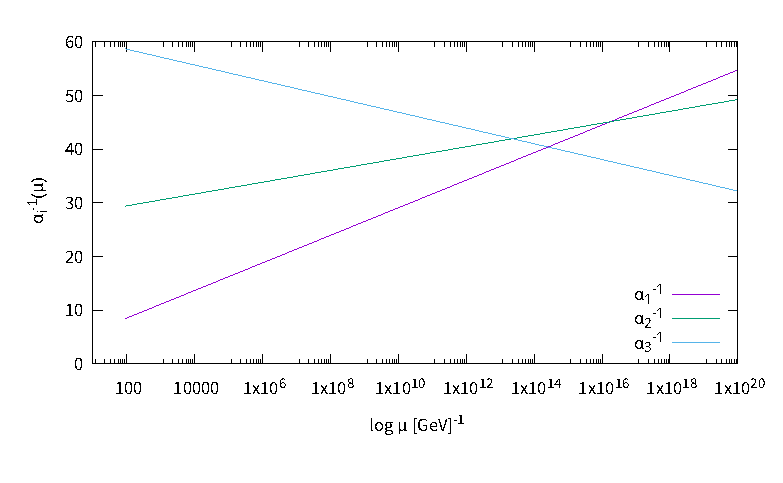
\includegraphics[width=12truecm,clip]{fig/RGE_SM.eps}
  \caption{標準模型粒子のみで繰り込み群方程式を解いた図}
  \label{fig:RGE_SM}
\end{figure}
%EOF


\chapter{場の理論における繰り込みと結合定数}
% ---------------------------------------
%
%  Renormalization and Running coupling constant
%  rge.tex
%  Program modified by Yasutoki Takamura
%  Last Modified Jan 22 2025
%
% ---------------------------------------
\section{走るゲージ結合定数}
場の量子論に基づけば, 理論に現れる発散を繰り込みという手法を用いて取り除くことが可能である.
\textcolor{red}{種類などもう少し細かい説明をするか?}

いずれの方法であってもエネルギースケールへ依存性があるが, 理論はエネルギーの変化に対して不変でなければならないため, ラグランジアンに存在するパラメータはエネルギースケールの変化を打ち消すように変化する.
これによってエネルギースケールに依存する繰り込まれた理論が得られる.
\section{Callan-Symanzik方程式}
繰り込まれた量子場の理論ではラグランジアンの項は制限が与えられ, 質量次元が4次の項のみ許される.
繰り込まれた場の理論のパラメータは, 繰り込み条件の組みで決定され, この条件が繰り込みスケールを決定している.
異なるエネルギースケールであっても同様の理論を考えることができる.

繰り込み条件を考えると, 繰り込みを行うスケール$M$は任意である.
したがって, 同じ理論を異なったスケール$M'$でも定義することができる.
このことを以下で考える. 

ある理論のグリーン関数が
\begin{align}
  \langle T \phi_0(x_1)\cdots\phi_0(x_n)\rangle  \label{rescale1}
\end{align}
で与えられるとする.
この理論では, 量子効果を考えない裸の結合定数$\lambda_0$や, 運動量カットオフが$\Lambda$によって与えられるものであり,エネルギースケール$M$には依存していない.
エネルギースケール依存性は, このグリーン関数にあるのではなく, 場をリスケーリングし裸の結合定数$\lambda_0$を消して繰り込まれた結合定数$\lambda$で書くことでカットオフ依存性を取り除いたときにのみ現れる.
繰り込まれたグリーン関数と裸のグリーン関数は, リスケーリング因子の$Z$に至るまでは数値的に同じになる.
場の繰り込みは場の強さの繰り込み因子である$Z$を用いて次のように定義される.
\begin{align}
  \phi(x) = Z^{-\frac{1}{2}}\phi_0(x) \label{bfnc-2}
\end{align}
これにより繰り込まれた$n$点の相関関数は, 裸の相関関数と次のように関係付けられる.
\begin{align}
  \langle T \phi(x_1)\cdots \phi(x_n)\rangle = Z^{-\frac{n}{2}}\langle T \phi_0(x_1)\cdots \phi(x_n)\rangle \label{bfnc-1}
\end{align}
式(\ref{bfnc-1})の左辺は繰り込まれたグリーン関数と呼ばれる.
この関数は右辺のグリーン関数とは異なる別のエネルギースケールである$M'$で定義されており, 結合定数は$\lambda'$, リスケーリング因子は$Z'$で定義される.

ここから, エネルギースケール$M$を無限小だけシフトした場合の影響を考える.
はじめに$G^{(n)}(x_1,\cdots,x_n)$を繰り込まれた摂動論において計算される連結$n$点関数とする.
\begin{align}
  G^{(n)}(x_1,\cdots,x_n) = \langle T\phi(x_1)\cdots\phi(x_n) \rangle_{\text{connected}}\label{rnpf}
\end{align}
繰り込みされていない裸の相関関数は, 繰り込みされていないパラメータである$(\phi_0,\lambda_0,m_0)$とカットオフ$\Lambda$に依存している.
一方で, 繰り込まれた相関関数(式(\ref{rnpf}))には繰り込まれたパラメーターである($\phi,\lambda,m)$と繰り込みスケール$\mu$に依存している.
このことから, 繰り込みされていない裸の相関関数$G^{(n)}_0$は繰り込みスケール$\mu$に依存せず, 繰り込みスケールの変化があった場合でも変化することがないので
\begin{align}
  \frac{d G_0^{(n)}}{d\mu} = 0 \label{bfnc-3}
\end{align}
が満たされる.
一方で, 繰り込まれた相関関数は繰り込みスケールが変化することで影響を受ける.
繰り込みスケールを無限小だけシフトする.
\begin{align}
  \mu\quad\rightarrow\quad \mu + \delta \mu \label{sftM}
\end{align}
このとき, 繰り込みスケールの変化に伴って$\lambda$と$\phi$は次のように変化する.
\begin{align}
  &\lambda \quad\rightarrow\quad \lambda + \delta \lambda \label{sftl}\\
  &\phi \quad\rightarrow\quad \phi+ \delta\phi \equiv (1+\delta\eta)\phi \label{sftp}
\end{align}
場の変換については無次元のシフトを$\delta \eta  = \frac{\delta\phi}{\phi}$とした.
式(\ref{bfnc-2})から
\begin{align}
  Z^{\frac{1}{2}} = 1 - \delta\eta\label{bfnc-4}
\end{align}
が言えるので, 式(\ref{bfnc-3})から繰り込みされた相関関数は
\begin{align}
  G^{(n)}\quad\rightarrow\quad(1+n\delta\eta)G^{(n)}\label{sftg}
\end{align}
と変化することがわかる.
これらを踏まえて, 繰り込みされた相関関数の微小変化を考えると, 式(\ref{bfnc-3})から
\begin{align}
  \frac{d}{d\mu} Z^{\frac{n}{2}}G^{(n)} = \frac{\partial G^{(n)}}{\partial \mu} + \frac{\partial G^{(n)}}{\partial \lambda}\frac{\partial \lambda}{\partial \mu} - n \frac{\partial \eta}{\partial \mu}G^{(n)} = 0
\end{align}
がわかるので, これを整理して
\begin{align}
  \left(\mu \frac{\partial}{\partial \mu} + \mu\frac{\partial \lambda}{\partial \mu} \frac{\partial}{\partial \lambda} -n\mu\frac{\partial \eta}{\partial \mu}\right)G^{(n)}(x_1,\cdots,x_n;\mu,\lambda) = 0\label{CS-1}
\end{align}
となる.
ここで無次元の量である$\beta$と$\gamma$を
\begin{align}
  &\beta = \mu\frac{\partial \lambda}{\partial \mu}\label{def_beta}\\
  &\gamma = -\mu\frac{\partial \eta}{\partial \mu} \label{def_gamma}
\end{align}
と定義すると, 次の関係式が得られる.
\begin{align}
  \left(\mu \frac{\partial }{\partial \mu} + \beta \frac{\partial}{\partial \lambda} + n \gamma\right) G^{(n)}(x_1,\cdots,x_n;\mu,\lambda) = 0 \label{bfnc-CS1}
\end{align}
式(\ref{bfnc-CS1})はCallan-Symanzik方程式と呼ばれる. \cite{callanBrokenScaleInvariance1970,symanzikSmallDistanceBehaviour1970,symanzikSmalldistancebehaviourAnalysisWilson1971}

Callan-Symanzik方程式に現れる$\beta, \gamma$の2つの関数はカットオフスケールの$\Lambda$に依存し, 繰り込みスケール$\mu$に依存しない.
つまり, この$\beta, \gamma$の2つの関数は次元を持たない繰り込まれた結合定数である$\lambda$の関数であることが言える.
これらは$G^{(n)}$にのみ繰り込みが行われているからである.

ここで新しく定義された$\beta, \gamma$の2つの関数は不変的な関数であり, 繰り込み定数と場の強さの変化にのみ依存しており, これらが変化したときの繰り込みスケール$\mu$の変化を補うように変化が起こる. 
そのため$\beta$関数は繰り込みスケールが$\mu$への結合定数の依存性を表し, 一方で$\gamma$関数は場を繰り込みスケール$\mu$への依存性を表している

次にCallan-Symanzik方程式に現れた新たな関数$\gamma$をを一般化し, 摂動との関係を考える.
$\delta \eta$は式(\ref{sftp})で定義されていた.
したがって,
\begin{align}
  \delta \eta &= \frac{Z^{-\frac{1}{2}}(\mu+\delta \mu)}{Z^{-\frac{1}{2}}(\mu)}-1\nonumber\\
              &= \frac{Z^{-\frac{1}{2}}(\mu+\delta \mu)-Z^{-\frac{1}{2}}(\mu)}{Z^{-\frac{1}{2}}(\mu)}
\end{align}
となる.
この両辺を$\delta \mu$で割り, $\delta \mu\rightarrow0$とすると
\begin{align}
  \frac{\partial \eta}{\partial \mu} = -\frac{1}{2}\frac{1}{Z}\frac{\partial Z}{\partial \mu}
\end{align}
一方で$\gamma$は式(\ref{def_gamma})で定義されているので,
\begin{align}
  \gamma = \frac{1}{2}\frac{\mu}{Z} \frac{\partial Z}{\partial \mu}\label{def_gamma_correct}
\end{align}
と$\gamma$の表し方を変えることができる.
ここから摂動論の関係を見ることができる.
摂動論を考えているとき, 場の強さ$Z$は
\begin{align}
  Z = 1 +\delta Z
\end{align}
と微小量$\delta Z \ll 1$を用いて書くことができる.
これより
\begin{align}
  \gamma \simeq \frac{1}{2}\mu \frac{\partial \delta Z}{\partial \mu} + \mathcal{O}((\delta Z)^2)
\end{align}
となる.
このことから摂動論が有効な理論であれば, $\delta Z$が判明すれば 相殺項から体系的に$\beta$関数を求めることができることがわかる.

ここまではCallan-Symanzik方程式をスカラー場の理論として式(\ref{rescale1})から導出した.
一般にフェルミオン場が存在した場合でも成り立つ.
$n$個のフェルミオン場, $m$個のスカラー場が存在し, 両方の結合定数が$\lambda$の場合を考える.
このとき, 場のくりこみを同じように考えると, 繰り込まれたグリーン関数は
\begin{align}
  G_0^{(n,m)}(\{x_i\},\lambda_0) = Z_\psi^{\frac{n}{2}} Z_\phi^{\frac{m}{2}}G^{(n,m)}(\{x_i\},\lambda,\mu)\label{renormalized_G}
\end{align}
となる.
したがって, 式(\ref{bfnc-3})と同じように考えて
\begin{align}
  \left(\mu\frac{\partial}{\partial \mu} + \beta\frac{\partial}{\partial \lambda} + n\gamma_\psi + m \gamma_\phi \right)G^{(n,m)}(\{x_i\},\mu,\lambda) = 0\label{renormalized_CS}
\end{align}
となる.
ここでは
\begin{align}
  \gamma_\psi = \frac{n}{2}\frac{\mu}{Z_\psi}\frac{\partial Z_\psi}{\partial \mu},\quad \gamma_\phi = \frac{m}{2}\frac{\mu}{Z_\phi}\frac{\partial Z_\phi}{\partial \mu}\label{def_gamma2}
\end{align}
とした.

これらより, 式(\ref{def_beta})
\begin{align}
  \beta \equiv \mu\frac{\partial}{\partial \mu}\lambda\nonumber
\end{align}
の$\beta$からゲージ結合定数$\lambda$のエネルギー依存性を求めることができる.
この$\beta$は摂動論において相殺項や繰り込まれたグリーン関数から求めることができ, 非可換ゲージ理論や湯川結合, スカラー場の理論など一般的な場の理論で同様に求めることができる.
\cite{chengHiggsPhenomenaAsymptotically1974,
machacekFermionHiggsMasses1981,
machacekTwoloopRenormalizationGroup1983,
machacekTwoloopRenormalizationGroup1984,
machacekTwoloopRenormalizationGroup1985,
maVariationMixingAngles1979,
vaughnRenormalizationGroupConstraints1982}
\section{ゲージ結合定数のエネルギー依存性}
式(\ref{def_beta})により, ゲージ結合定数のエネルギー依存性を$\beta$関数によって導くことができることが明らかにされた.
理論に現れる相殺項を求めることで$\beta$-関数の具体的な形を求めることができるが, 群論の対称性を用いることで一般的な$\beta$-関数の係数は導出されている.
摂動の$\delta Z$の1次の影響まで考えた場合,
\begin{align}
  \beta = -\frac{g^3}{(4\pi)^2}\left[\frac{11}{3}C_2(G) -\frac{4}{3}\kappa S(F) - \frac{1}{6}\eta S(S)\right]
\end{align}
となる.
\footnote{
本論文では扱わないが, 2次までの摂動の計算をすると次のようになる.
\cite{caswellAsymptoticBehaviorNonAbelian1974,jonesTwoloopDiagramsYangMills1974,jonesTwoLoopBeta1982}
\begin{align}
  \beta &= -\frac{g^3}{(4\pi)^2}\left[\frac{11}{3}C_2(G) -\frac{4}{3}\kappa S_2(F) - \frac{1}{6}\eta S_2(S)\right] \nonumber\\
        &\quad-\frac{g^5}{(4\pi)^4}\left[ \frac{34}{3}[C_2(G)]^2 -\kappa\left(4C_2(F)+\frac{20}{3}C_2(G)\right)S_2(F) -\left(2C_2(S)+\frac{1}{3}C_2(G)\right)\eta S_2(S)\right] \nonumber
\end{align}
}
\cite{grossUltravioletBehaviorNonAbelian1973,politzerReliablePerturbativeResults1973}

多重項は群$G$の表現$R$によって変換される.
ここではフェルミオン多重項であれば群$G$の表現$F$によって, ボゾン多重項は群$G$の表現$S$によって変換する.
ここでは,$C_2(R)$は
$\kappa$ $\eta$はそれぞれ
\begin{align}
  \kappa = \left\{\begin{array}{cc}
      1 & ディラックフェルミオン \\
      \cfrac{1}{2} & ワイルフェルミオン
    \end{array}\right.,\quad
  \eta = \left\{\begin{array}{cc}
      1 & 実スカラー場\\
      2 & 複素スカラー場
    \end{array}\right. \nonumber
\end{align}
と対応づけられる.
また, $S_2(F), S_2(S)$はそれぞれフェルミオン表現とスカラー表現のDynkin指数である.
群$G$の生成子の表現行列を$T^a$とする.
これは交換関係(\ref{gauge-1})を満たす.
この表現行列$T^a$は次の関係を満たす.
\begin{align}
  T^a T^a &= C_2(R)I\nonumber\\
  \mathrm{Tr}[T^a T^b] &= S_2(R)\delta^{ab}\nonumber
\end{align}
ここで$I$は単位行列である.
$C_2(R)$はカシミア演算子と呼ばれ, 群$G$の生成子と交換する.
\begin{align}
  d(G)S_2(R) = d(R)C_2(R)
\end{align}
ここで, $d(R)$は$R$の次元であり, $d(G)$はゲージ群$G$の随伴表現の次元である.
随伴表現の次元は群の次元と等しい.

ここで$b_i$を
\begin{align}
  b_i &= -\frac{11}{3}C_2(G) +\frac{4}{3}\kappa S_2(F) + \frac{1}{6}\eta S_2(S)\nonumber
\end{align}
とし, $i=1,2,3$はそれぞれ$U(1)_Y, SU(2)_L, SU(3)_c$ゲージ群と対応する.
また, 後述される式(\ref{re_gY})によって$U(1)_Y$ゲージ結合定数は$g_1^2\equiv \sqrt{\frac{5}{3}}g_Y$と規格化される.
標準模型では
\begin{align}
  \left(b_1, b_2, b_3 \right) = \left( \frac{41}{10}, -\frac{19}{6}, -7\right)\nonumber
\end{align}
と係数を求めることができる.
ここから実際に数値的にゲージ結合定数の大きさについて, エネルギー依存性を見る.
\begin{figure}[ht]
  \centering
  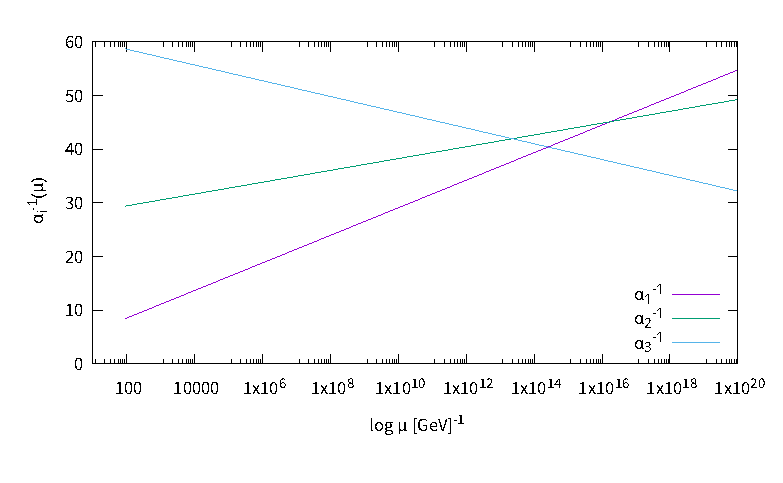
\includegraphics[width=12truecm,clip]{fig/RGE_SM.eps}
  \caption{標準模型粒子のみで繰り込み群方程式を解いた図}
  \label{fig:RGE_SM}
\end{figure}
$\alpha_i$は$\alpha_i(\mu) = \cfrac{g_i(\mu)}{4\pi}$として, 式(\ref{def_beta})に代入し, 
\begin{align}
  \frac{d \alpha_i^{-1}(\mu)}{d\,\mathrm{ln}{\mu}} = -\frac{1}{2\pi}b_i
\end{align}
とする.
電弱スケール $M_Z=91.1880\,[\mathrm{GeV}]$におけるゲージ結合定数の値は
\begin{align}
  g_1(M_Z) &= 0.461\nonumber\\
  g_2(M_Z) &= 0.652\nonumber\\
  g_3(M_Z) &= 1.22\nonumber
\end{align}
であり
\cite{navasReviewParticlePhysics2024}, これらを初期条件として数値的に解いたものが図\ref{fig:RGE_SM}となる.
図\ref{fig:RGE_SM}を見ると明らかであるが, 高エネルギースケールでゲージ結合定数の大きさは近づくものの, 完全には一致しない.
しかし, いずれの相互作用の大きさもプランクスケールである$M_{pl}\sim 10^{19}\,[\mathrm{GeV}]$よりも下で近づくため, 3つの相互作用は重力相互作用よりも先に統一される可能性は残されている.

%EOF


\chapter{素粒子標準模型では説明できない物理}
% ---------------------------------------
%
%  Some difficulties of Standard Model
%  SM_problems.tex
%  Program modified by Yasutoki Takamura
%  Last Modified Jul 18 2024
%
% ---------------------------------------
\section{標準模型の抱える問題}
素粒子標準模型は高エネルギー物理学の実験をほぼ正確に予言することができるため, 大きな成功を収めた.
特に2011年にCERNにある大型ハドロン衝突型加速器(Large Hadron Corrider; LHC)が標準模型に現れるHiggs粒子を発見したことにより, 標準模型は揺るぎないものとなった.
しかし, 次のような課題があり, 理論の拡張が迫られている.
\begin{itemize}
        \item ニュートリノ質量, およびニュートリノ振動\\
              標準模型ではニュートリノは質量を持たない粒子として存在する.
              しかし1998年にニュートリノ振動がスーパーカミオカンデで観測されたことにより, ニュートリノは質量を持つことが示唆されたため, 標準模型を何かしら拡張する必要があると考えられている.
      \item 重力相互作用
      \item 真の統一理論
      \item 電荷の量子化
      \item 階層性問題
      \item 予言できないパラメーターの数
      \item 暗黒物質
      \item 暗黒エネルギー
\end{itemize}
%EOF



\section{ニュートリノ質量}
% ---------------------------------------
%
%  Neutrino Mass
%  neutrino.tex
%  Program modified by Yasutoki Takamura
%  Last Modified Jan 08 2025
%
% ---------------------------------------
$BAGN3;RI8=`LO7?$G$O(B, $B%K%e!<%H%j%N$K$O<ANL$,$J$$(B.
$B$3$l$O(B, $B%l%W%H%s%;%/%?!<$G$O%K%e!<%H%j%N$O(B$SU(2)_L$$BFs=E9`$K$N$_B8:_$7(B, $B%+%$%i%k%Q!<%H%J!<$G$"$k1&4,$-%K%e!<%H%j%N$,B8:_$;$:(B, $BB>$NN3;R$N$h$&$K%R%C%0%95!9=$r9M$($k$3$H$,$G$-$J$$$?$a$G$"$k(B.
$B$H$3$m$,(B, $B$9$G$K%+%_%*%+%s%G$K$h$k4QB,$K$h$j(B, $B%K%e!<%H%j%N?6F0$H8F$P$l$k%K%e!<%H%j%N$N%U%l!<%P!<$,JQ2=$9$k8=>]$,H/8+$5$l$?$3$H$+$i%K%e!<%H%j%N$K$b<ANL$,$"$k$H9M$($J$1$l$P$J$i$J$$(B.
\subsection{$B%^%h%i%J%U%'%k%_%*%s$H<ANL9`(B}
$B$3$3$G$O(B, $B%K%e!<%H%j%N$N<ANL9`$rF3F~$9$k$?$a$K%^%h%i%J>l$rF3F~$9$k(B.
$BNL;R>l$NM}O@$G$O(B, $B<ANL$r;}$C$?N3;R$O(B4$B@.J,$N%G%#%i%C%/%9%T%N!<%k>l$rMQ$$$F5-=R$5$l$F$$$?(B.
$B$3$N%G%#%i%C%/%9%T%N!<%k>l$r(B$\psi_D$$B$H$9$k(B.
$B%G%#%i%C%/%9%T%N!<%k$H%+%$%i%k%9%T%N!<%k$K$O<M1F1i;;;R(B$P_L = \cfrac{1-\gamma^5}{2}$, $P_R = \cfrac{1+\gamma^5}{2}$$B$rMQ$$$F<!$N$h$&$K<($5$l$k(B.
\begin{align}
  \psi_R = P_R \psi,\quad \psi_L = P_L \psi\nonumber
\end{align}
4$B@.J,%9%T%N!<%k>l(B$\psi$$B$O(B2$B$D$N%+%$%i%k%9%T%N!<%k$NOB$G=q$/$3$H$,$G$-$k(B.
\begin{align}
  \psi &= \psi_L + \psi_R\nonumber\\
       &= \frac{1+\gamma^5}{2}\psi + \frac{1-\gamma^5}{2}\psi\nonumber\\
       &= P_L\psi + P_R\psi\label{Mj_1}
\end{align}
$B$3$3$+$i(B, $\gamma$$B9TNs$O%+%$%i%k4pDl$r$H$k(B.
$B$3$l$K$h$C$F%+%$%i%k%9%T%N!<%k$r(B2$B@.J,$N%9%T%N!<%k$H$7$F07$&$3$H$,$G$-$k(B.
$B6qBNE*$K$O(B,$B%Q%&%j9TNs(B$\sigma^{i}\,(i=1,2,3)$$B$KBP$7$F(B
\begin{align}
  \sigma ^\mu &= ( I, \sigma^i )\nonumber\\
  \bar{\sigma} ^\mu &= (I, -\sigma^i ) \nonumber
\end{align}
$B$HDj5A$9$k$H(B, 
$\gamma$$B9TNs$O(B
\begin{align}
  \gamma ^{\mu} = \left(\begin{array}{cc}
                             0 &  \sigma ^{\mu}     \\
                             \bar{\sigma}^{\mu} & 0 \\
                           \end{array}
                           \right)
\end{align}
$B$H=q$/$3$H$,$G$-$k(B.
$B$3$N$3$H$+$i(B, $B%+%$%i%k%9%T%N!<%k$O(B
\begin{align}
  \psi_L = \left( \begin{array}{c}
                   \eta_\alpha \\
                   0 \\
                 \end{array}
                 \right);\,\,(\alpha =1,2)\nonumber\\
  \psi_R = \left(\begin{array}{c}
                   0 \\
                   \bar{\xi}^{\dot{\alpha}} \\
                 \end{array}
           \right);\,\,(\dot{\alpha} = 1,2)
\end{align}
$B$H$J$j(B, $B$=$l$>$l(B2$B@.J,$NJ#AG%Y%/%H%k$GI=$9$3$H$,$G$-$k(B.
$B$^$?(B, $B%m!<%l%s%D72$N@8@.;R(B$\sigma^{\mu\nu}$$B$O(B
\begin{align}
  \Sigma ^{\mu\nu} = \frac{i}{2}\left(\begin{array}{cc}
      \sigma ^{\mu\nu} & 0 \\
                             0                & \bar{\sigma}^{\mu\nu} \\
                           \end{array}
                         \right),\qquad(\sigma^{\mu\nu}\equiv \sigma^\mu\bar{\sigma}^\nu,\quad\bar{\sigma}^{\mu\nu}\equiv\bar{\sigma}^\mu\sigma^\nu\quad(\mu\neq\nu))
\end{align}
$B$H$J$j(B, $B%m!<%l%s%DJQ49$N2<$G0[$J$k%+%$%i%j%F%#$r;}$D>l$,:.9g$7$J$$(B.
$B?t3XE*$K$O72(B$SL(2,\mathbb{C})$$B$N4{LsI=8=$r@.$9$3$H$,L@3N$K$J$k(B.

$B%+%$%i%k4pDl$G$O(BC$BJQ49$O(B $C = i\gamma^0\gamma^2$$B$H9TNs$GI=$9$3$H$,$G$-$?(B.
$B$3$l$h$j%+%$%i%k%U%'%k%_%*%s$O(B
\begin{align}
  (\psi_L)^c &= C\bar{\psi}_L^t = -i\gamma^2 (\psi_L)^*\nonumber\\
             &= \left(\begin{array}{c}
                        0 \\
                        \bar{\eta}^{\dot{\alpha}}
                      \end{array}\right)
\end{align}
$B$H0[$J$k%+%$%i%j%F%#$r;}$D%+%$%i%k%U%'%k%_%*%s$r9=@.$9$k$3$H$,$G$-$k(B.

$B$3$l$^$G$G(B, $B%G%#%i%C%/%9%T%N!<%k$O(B
\begin{align}
  \psi_D = \psi_L + \psi_R = \left(\begin{array}{c}
                                  \eta_\alpha \\
                                  \bar{\xi}^{\dot{\alpha}}
                                \end{array}
                                \right)
\end{align}
$B$HI=$;$k(B.
$B$5$i$K(B, C$BJQ49$O%+%$%i%j%F%#$rJQ2=$5$;$k$3$H$+$i(B, $B$"$k:84,$-$N%+%$%i%k%U%'%k%_%*%s$H$=$NH?N3;R$G%9%T%N!<%k$r9=@.$9$k$3$H$,2DG=$G$"$k$3$H$,$o$+$k(B.
\begin{align}
  \psi_{ML} = \psi_L + (\psi_L)^c = \left(\begin{array}{c}
                                  \eta_\alpha \\
                                  \bar{\eta}^{\dot{\alpha}}
                                \end{array}
                                \right)
\end{align}
$B$"$k$$$O1&4,$-$N%+%$%i%k%U%'%k%_%*%s$rMQ$$$k$H(B
\begin{align}
  \psi_{MR} = \psi_R + (\psi_R)^c = \left(\begin{array}{c}
                                  \xi_\alpha \\
                                  \bar{\xi}^{\dot{\alpha}}
                                \end{array}
                                \right)
\end{align}
$B$N$h$&$K(B, $B%9%T%N!<%k$r9=@.$9$k$3$H$,2DG=$H$J$k(B.
$B$3$N$h$&$K$7$F9=@.$5$l$?%9%T%N!<%k$O%^%h%i%J%9%T%N!<%k$H8F$P$l$k(B.

$B%^%h%i%J%9%T%N!<%k$N=EMW$JE@$H$7$F(B, P$BJQ49$H(BC$BJQ49$r(B2$B2s;\$9$H85$N>uBV$KLa$k(B.
$B0J>e$N$3$H$+$i(B, $B%^%h%i%J%9%T%N!<%k$ON3;R$HH?N3;R$N6hJL$,$J$$Cf@-$N%U%'%k%_%*%s$rI=$9(B.

$B$3$3$G(B, $B?t3XE*$JB&LL$K8@5Z$9$k(B.
$\eta, \bar{\xi}$ $B$O%m!<%l%s%D72(B$SL(2,\mathbb{C})$$B$N4pK\I=8=$H$=$NH?I=8=$H$7$F$N?6$kIq$$$r$9$k(B.
$B$3$l$i$O(BLevi-Civita$B%F%s%=%k$rMQ$$$F(B
\begin{align}
  \bar{\eta}^{\dot{\alpha}} = \epsilon^{\dot{\alpha}\dot{\beta}}\bar{\eta}_{\dot{\beta}}
\end{align}
$B$H$J$j(B, Levi-Civita$B%F%s%=%k$,7WNL$H$7$F$NLr3d$r;}$D(B.

$B$3$3$G(B, $BG$0U$N(B2$B$D$N:84,$-%9%T%N!<%k(B$\eta, \chi$$B$N=LLs$r9M$($k(B.
\begin{align}
  \eta_\alpha \chi ^\alpha = \epsilon^{\alpha\beta}\eta_\alpha \chi_\beta \nonumber
\end{align}
$B$O(B$SL(2,\mathbb{C})$$BJQ49$N$b$H$GITJQ$G$"$k$+$i(B, $B%m!<%l%s%DITJQNL$G$"$k$3$H$,$o$+$k(B.
$B$3$l$O(B$SU(2)$$B72$K$*$$$F4pK\I=8=$N(B2$B=E9`$rH?BP>N$KAH$`$3$H$K$h$C$F(B1$B=E9`$r@.$7(B, $SU(2)$$BITJQNL$r@.$9$3$H$rI=$7$F$$$k(B.
\footnote{$B$3$l$O;~6u$r%_%s%3%U%9%-!<E*$G$O$J$/%f!<%/%j%C%IE*$H$9$k$H(B, $B%m!<%l%s%DJQ49$,(B$SO(4)\simeq SU(2)\times SU(2)$$B$H$J$j(B, $BFHN)$J(B$SU(2)$$B$G5-=R$G$-$k$3$H$HBP1~$7$F$$$k(B.}

$B%^%h%i%J%9%T%N!<%k$N9=@.$r9T$C$?$3$H$K$h$j(B, $B%^%h%i%J7?$N<ANL9`$r9=@.$9$k$3$H$,$G$-$k(B.
\begin{eqnarray}
  -m_L \overline{\psi_{ML}}\psi_{ML} = -m_L(\overline{\nu_L^c}\nu_L +\mathrm{h.c.}) = m_L(\eta^\alpha \eta_\alpha + \mathrm{h.c.})\label{Mj_L}\\
  -m_R \overline{\psi_{MR}}\psi_{MR} = -m_R(\overline{\nu_R^c}\nu_R +\mathrm{h.c.}) = m_R(\xi^\alpha \xi_\alpha + \mathrm{h.c.})\label{Mj_R}
\end{eqnarray}
$B0lJ}$G(B, $B:84,$-%K%e!<%H%j%N$N%+%$%i%k%Q!<%H%J!<$H$7$F1&4,$-$N%K%e!<%H%j%N$rM}O@$K4^$a$?$3$H$K$h$j(B, $BB>$N%U%'%k%_%*%s$HF1$8$h$&$K%G%#%i%C%/7?$N<ANL9`$r9M$($k$3$H$,$G$-$k(B.
\begin{eqnarray}
  -m_D\bar{\psi_D}\psi_D = -m_D(\bar{\psi_L}\psi_R + \bar{\psi_R}\psi_L)\label{D_n}
\end{eqnarray}
$B$3$l$i$r$^$H$a$k$H(B, $B%K%e!<%H%j%N$N<ANL9`$O<0(B(\ref{Mj_L}), (\ref{Mj_R}), (\ref{D_n})$B$rMQ$$$F(B, $B0lHLE*$K(B
\begin{eqnarray}
  \mathcal{L}_{\mathrm{mass}} = -\frac{1}{2}m_L(\overline{\nu_L^c}\nu_L +\mathrm{h.c.}) -\frac{1}{2}m_R(\overline{\nu_R^c}\nu_R +\mathrm{h.c.}) -m_D(\bar{\nu_L}\nu_R + \bar{\nu_R}\nu_L)\label{Lagrangian_nMass}
\end{eqnarray}
$B$HI=$9$3$H$,$G$-$k(B.

$B$3$3$G(B, $B<0(B(\ref{Lagrangian_nMass})$B$r9TNs$G$^$H$a$k(B.
\begin{eqnarray}
  \mathcal{L}_{\mathrm{mass}} = -\frac{1}{2}\left( 
  \begin{array}{cc}
    \overline{(\nu_L)^c} & \overline{\nu_R}
  \end{array}\right)
        \left( \begin{array}{cc}
        m_L & m_D \\
        m_D & m_R 
    \end{array}\right)
    \left( \begin{array}{c}
     \nu_L  \\
     (\nu_R)^c \end{array}\right)
     + \mathrm{h.c.}\label{Lagrangian_mt_nMass}
\end{eqnarray}
$B0lHLE*$K<ANL9TNs$OJ#AG9TNs$G$"$k(B.
$B$3$N$H$-(B, $BJ#AGBP>N9TNs$O%f%K%?%j!<9TNs$H$=$NE>CO9TNs$K$h$jBP3Q2=$9$k$3$H$,$G$-$k(B.
\begin{eqnarray}
  \left( \begin{array}{cc}
        m_L & m_D \\
        m_D & m_R 
    \end{array}\right)
 =
  U^T\left( \begin{array}{cc}
        m_a & 0 \\
          0 & m_s 
    \end{array}\right)U
\end{eqnarray}
$B$3$N$H$-(B, $BBP3Q2=9TNs(B$U$, $\nu_L$$B$H(B$(\nu_R)^c$$B$N:.9g3Q(B$\theta_\nu$$B$O$=$l$>$l(B
\begin{eqnarray}
  U =\left(
  \begin{array}{cc}
        -i\cos\theta_\nu & \sin\theta_\nu  \\
         i\sin\theta_\nu & \cos\theta_\nu
     \end{array}\right),\quad \tan2\theta_\nu = \frac{2m_D}{m_R-m_L}
\end{eqnarray}
$B$H$J$k(B.
$B<ANL8GM->uBV$H%+%$%i%k8GM->uBV$O(B
\begin{eqnarray}
  \left(\begin{array}{c}
      \nu_a \\
      \nu_s
    \end{array}
    \right) = U^\dagger
  \left(\begin{array}{c}
      \nu_L \\
      (\nu_R)^c
    \end{array}
    \right)
\end{eqnarray}
$B$H$$$&4X78$H$J$k(B.

$B0J>e$K$h$j(B2$B$D$N<ANL8GM-CM(B$m_a$, $m_s$$B$H$=$l$>$l$N<ANL8GM->uBV(B$\nu_a$, $\nu_s$$B$rF@$k$3$H$,$G$-$k(B.
\begin{eqnarray}
  m_a &=& \frac{1}{2}\left[ \sqrt{(m_R - m_L)^2 + 4m_D^2} - (m_R+m_L)\right]\nonumber\\
  m_s &=& \frac{1}{2}\left[ \sqrt{(m_R - m_L)^2 + 4m_D^2} + (m_R+m_L)\right]\nonumber\\
  \nu_a &=& i\left(\nu_L\cos\theta_\nu - (\nu_R)^c\sin\theta_\nu\right)\nonumber\\
  \nu_s &=& \nu_L\sin\theta_\nu + (\nu_R)^c\cos\theta_\nu\nonumber
\end{eqnarray}
$B<ANL8GM->uBV(B$\nu_a$$B$H(B$\nu_s$$B$K$h$C$F(B, 1$B$D$N@$Be$+$iFHN)$J(B2$B$D$N%^%h%i%J%U%'%k%_%*%s$N<ANL9`$r=q$/$3$H$,$G$-(B,
\begin{eqnarray}
  \mathcal{L} = -\frac{1}{2}m_s\bar{\nu_s}\nu_s -\frac{1}{2}m_a\bar{\nu_a}{\nu_a} + \mathrm{h.c.}
\end{eqnarray}
$B$H$J$k(B.
$B$3$3$^$G$G%^%h%i%J%U%'%k%_%*%s$H%G%#%i%C%/%U%'%k%_%*%s$+$i%K%e!<%H%j%N$N<ANL9`$r0lHLE*$KF3$/$3$H$r9T$C$?(B.
$B%K%e!<%H%j%N$,<ANL$r;}$D5!9=$K$D$$$F$O$$$/$D$+9M$($i$l$F$*$j(B, $B<g$K(B
\begin{itemize}
  \item $B%G%#%i%C%/7?(B$\cdots$$B%^%h%i%J<ANL$r;}$?$:$K%G%#%i%C%/7?$N<ANL9`$N$_$r9M$($k(B.
  \item $B%7!<%=!<5!9=(B$\cdots$$B%G%#%i%C%/<ANL$h$jHs>o$KBg$-$J%^%h%i%J<ANL$,B8:_$9$k(B.
  \item $B5<%G%#%i%C%/!&%K%e!<%H%j%N(B$\cdots$$B%G%#%i%C%/<ANL$h$jHs>o$K>.$5$J%^%h%i%J<ANL$,B8:_$9$k(B.
\end{itemize}
$B$,Ds0F$5$l$F$$$k(B.
$B$3$NCf$G$b%7!<%=!<5!9=$O%K%e!<%H%j%N$,B>$N%U%'%k%_%*%s$KHf$Y$FHs>o$K>.$5$J<ANL$r;}$D$3$H$r<+A3$K@bL@$9$k$3$H$,$G$-$k(B.
\subsection{$B%7!<%=!<5!9=(B}



% ----------------------------------------
%
%  Grand Unified Theory
%  grand_unified_theory.tex
%  Program modified by Yasutoki Takamura
%  Last Modified Jan 20 2025
%
% ----------------------------------------
\chapter{SU(5)大統一理論}
大統一理論はH.GeorgiとS.L.Glashowにより1974年に提唱された\cite{PhysRevLett.32.438}.
大統一理論では重力を除いた3つの相互作用を1つに統一することを目的としている.
したがって, ゲージ対称性は単純群によって記述されると考えられており, 標準模型のゲージ群である$\mathcal{G}_\text{SM}= SU(3)_c\times SU(2)_L\times U(1)_Y$を部分群として内包する群を考える.
このことから, 前節で述べられている標準模型の問題点のうち,
\begin{itemize}
  \item 電荷の量子化
  \item 予言できないパラメータの数
\end{itemize}
は大統一理論によって解決される可能性がある.

大統一理論にも様々な単純群を考えることが可能であり, $SU(5)$や$SO(10)$, $E_6$などの模型を考えることが可能であるが, このノートでは最小模型である$SU(5)$について取り扱い, 理論の拡張を試みる.

はじめに, $SU(5)$大統一理論が最小模型である理由を考える.
標準模型のゲージ対称性である$SU(3)_c\times SU(2)_L\times U(1)_Y$は, 群の階数が$\text{rank}=4$であり, これを内包できる群を考える必要がある.
その中で考えられる単純群は, $\text{O}(8)$, $\mathrm{O}(9)$, $\mathrm{Sp}(8)$, $\mathrm{F}_4$, そして $\mathrm{SU}(5)$である.
このうち, $SU(3)$のもつ3重項をもち, $SU(2)$がもつ2重項の複素表現をもつという性質は$SU(5)$群を用いて記述することができるため, 最小模型として$SU(5)$群を考えて理論を構築することが可能となる.

%\section{Georgi-Glashow モデル}
\section{フェルミオンの表現}
ここでは$SU(5)$群において標準模型に現れるフェルミオンがどのように当てはめられるのか考える.

ゲージ群を決定すると, ラグランジアンに導入する場の既約表現を指定すれば理論を定めることができる.
$SU(5)$の基本表現は$5$表現であり, $5$表現か, その複素表現である$\overline{5}$を用いることですべての表現を構成することができる.
$SU(5)$群の階数は4であるから, 生成演算子を$L_i$$(i=1,\cdots,24)$ のうち対角化可能なものが4つ存在する.
$SU(3)_c$の対角化可能な生成演算子を$\lambda_3,\lambda_8$, $\mathrm{SU}(2)$のものを$I_3$ (アイソスピン), $U(1)$の超電荷を$Y$に対応させて考えることができる.

次にフェルミオンの次元を$\mathrm{SU}(3), \mathrm{SU}(2)$の表現次元, $U(1)$の超電荷$Y$で $(1, 2, -1)$のように表し, どのように$SU(5)$模型に当てはめられるか考える.
\begin{center}
\begin{tabular}{clc}
             &                         & 多重度 \\
  $(u, d)_L$ & $(3  , 2, \frac{1}{6})$ &      6 \\
    $d_L^c $ & $(3^*, 1, \frac{1}{3})$ &      3 \\ 
    $u_L^c $ & $(3^*, 1,-\frac{2}{3})$ &      3 \\ 
$(\nu, e)_L$ & $(1  , 2,-\frac{1}{2})$ &      2 \\ 
     $e_L^c$ & $(1  , 1,           1)$ &      1 \\ 
   $\nu_L^c$ & $(1  , 1,           0)$ &      1 \\ 
\end{tabular}
\end{center}

基本表現をこの中から選ぶことで
\begin{align}
  (q_L^c, \nu_L, e_L) = (3^*, 1, Y)\oplus\left(1,2,-\frac{1}{2}\right) = \overline{5}
\end{align}
と考えられる.
ここではまだ$q$の正体が$u, d$クォークのどちらかは定かではないが, $\mathrm{SU}(5)$群のトレースは0でなければならないため, $Q$を電荷とすると上記の電荷は
\begin{align}
  \sum_{a=1}^5 Q_a = 3Q_{qc}+Q_\nu + Q_e\nonumber\\
  \therefore\quad Q_q = -Q_{qc} = -\frac{1}{3}\label{quantum_Q}
\end{align}
となる.
したがって, $q=d$と選択することにより, 次のように$\bm{5}$表現を決めることができる.
\begin{align}
 \psi_{\overline{\bm{5}}} =\begin{pmatrix}
    d_1 ^c \\
    d_2 ^c \\
    d_3 ^c \\
    l      \\
    -\nu_l
  \end{pmatrix}=\left({3}^*,1,\frac{1}{3}\right)\oplus \left(1,2,-\frac{1}{2}\right)\label{GUT-5rep}
\end{align}
これによりクォークの電荷が荷電レプトンの$\frac{1}{3}$の整数倍となっていることが説明できる.
残りのフェルミオンを次元の大きい表現に当てはめることを考える.
基本表現よりも大きな表現は, すべて基本表現の積で表すことができる.
${\bm{10}}$表現は
\begin{align}
  \bm{5}\otimes\bm{5} = \bm{15}\oplus\bm{10}\nonumber
\end{align}
として構成することができる.
この$\bf{10}$表現は$\bm{10}\rightarrow (3^*,1,-\frac{2}{3})\oplus(3,2,\frac{1}{6})\oplus(1,1,1)$
と分解できるので, 次のように当てはめることができる.
\begin{align}
\psi_{{\bm{10}}} = \frac{1}{\sqrt{2}}\begin{pmatrix}
         0 &  u_3^c & -u_2^c & u_1 & d_1 \\
    -u_3^c &      0 &  u_1^c & u_2 & d_2 \\
     u_2^c & -u_1^c &      0 & u_3 & d_3 \\
    -u_1   &   -u_2 &   -u_3 &   0 & e^c \\
      -d_1 &   -d_2 &   -d_3 &-e^c &   0 \\
    \end{pmatrix}\label{GUT-10rep}
% Note
% 10表現であれば内部に規格化定数を入れる場合があるがここで必要ではないのか確認しなければならない.
% Dec 10: up quark massを出す際に規格化されている必要があるので, この規格化定数は必要.
\end{align}
ただし, $x^c$は$x$を同じカイラリティで荷電共役したものを表している.
この$x$の例として, 左巻きの電子$e^-_L$を考える.
$e^-_L$に対して荷電共役変換を行った$(e^-_L)^c$を考える.
これは右巻きの電子$e_R^-$となるが, 左巻きの陽電子である$e_L^+$と同じである.
\section{ゲージ粒子の表現}
ゲージ粒子を$SU(5)$大統一理論で考えるために, 群の生成子について考える.
一般に$SU(n)$ゲージ群の変換は, 
\begin{align}
  U =\exp\left(-i \sum_{i=1}^{n^2-1}\beta_i L_i\right)=\exp(-\bm{\beta}\cdot \bm{L})
\end{align}
で表される.
ここで, $L_i$は群の生成子であり, エルミート性があり, トレースレス($\mathrm{tr} L_i =0$)である.
これにより$U$はユニタリーであり, $\mathrm{det}U =1$を満たす.
$L_i$は
\begin{align}
  \mathrm{tr}(L_iL_j) = \frac{1}{2}{\delta_{ij}}\label{reguralization}
\end{align}
と規格化する.
ここで, 表現行列を昇降演算子との類推で今後のために
\begin{align}
  (L^a_b)^c_d \equiv \delta^c_b\delta^a_d -\frac{1}{n}\delta^a_b\delta^c_d,\quad ((L^a_b)^\dagger=L^b_a)
\end{align}
と定義する.
交換関係は
\begin{align}
  [L^a_b,L^c_d] = \delta^a_bL^c_b - \delta^c_bL^a_d
\end{align}
を満たす.
これまで$n$表現について考えたが, 共役な表現$\overline{n}$を考えた場合,
\begin{align}
  L^a_b(\overline{n}) = -L^{aT}_b = -L^b_a
\end{align}
を満たす.

ここから具体的にゲージ場について考える.
$SU(n)$ゲージ理論では, $n^2-1$個のゲージ場が存在する.
これらは随伴表現で表される.
$SU(5)$群の生成演算子をこれまでのように$[L_i]^a_b\,(i=1,\cdots,24, a,b=1,\cdots,5)$として構成する.
基本表現である$5$表現の類推からは$a,b=1,2,3$はカラー量子数, $a,b=4,5$がアイソスピン量子数と考えられる.
そのため$i=1,\cdots,8$を$SU(3)$部分, $i=9,10,11$を$SU(2)$の部分群として考えると
\begin{align}
  L_i(i=1,\cdots,8) = \left(\begin{array}{@{}c|c@{}}
      \mbox{$\cfrac{1}{2}\lambda_i$} &
      \begin{matrix}
        0 & 0 \\
        0 & 0 \\
        0 & 0 
      \end{matrix}\\
      \hline
      \begin{matrix}
        0 & 0 & 0\\
        0 & 0 & 0
      \end{matrix} &{\large{\mbox{$0$}}}
  \end{array}\right),\quad
  L_i(i=9,10,11) = \left(\begin{array}{@{}c|c@{}}
      \mbox{\Large 0} &
      \begin{matrix}
        0 & 0 \\
        0 & 0 \\
        0 & 0 
      \end{matrix}\\
      \hline
      \begin{matrix}
        0 & 0 & 0\\
        0 & 0 & 0
      \end{matrix} & {\mbox{$\cfrac{1}{2}\sigma_j$}}
  \end{array}\right)
\end{align}
ただし, $\sigma_{j=i-8}\,(j=1,2,3)$である.

対角行列は$L_3, L_8, L_{11}$にそれぞれ$SU(3), SU(2)$群の対角行列を対応させる.
残りの1つは$L_{12}$であり, $U(1)_Y$の超電荷を対応させる.
基本表現である$\bm{5}$表現の超電荷を対応させ, 規格化条件である式(\ref{reguralization})を用いることで
\begin{align}
  L_{12}=\frac{1}{2\sqrt{15}}\mathrm{diag}(-2,-2,-2,3,3)\nonumber
\end{align}
と決めることができる.


24個のゲージボゾンは随伴表現として存在し, 次のように分解できる.
\begin{align}
  \bm{24} = G(8,1,0)\oplus W(1,3,0)\oplus B(1,1,0)\oplus \overline{X}(3,\bar{2},-\frac{5}{6})\oplus X(\bar{3},2,+\frac{5}{6})
\end{align}
ゲージボゾンを$V_\mu$とすると,
\begin{align}
  \frac{1}{\sqrt{2}}V_\mu &= \sum_{i=1}^{24}\frac{1}{2}V_\mu^i L_i\\
  V_\mu &= \left(\begin{array}{ccccc}
    G^1_1 - \frac{2B}{\sqrt{30}} & G^1_2 & G^1_3 & \overline{X_1} & \bar{Y_1} \\
    G^2_1 & G^2_2 - \frac{2B}{\sqrt{30}} & G^2_3 & \overline{X_2} & \bar{Y_2} \\
    G^3_1 & G^3_2 & G^3_3 - \frac{2B}{\sqrt{30}} & \overline{X_3} & \bar{Y_3} \\
    X_1   & X_2 & X_3 & \frac{W^3}{\sqrt{2}} + \frac{3B}{\sqrt{30}} & W^+ \\
    Y_1   & Y_2 & Y_3 & W^- &    -\frac{W^3}{\sqrt{2}} + \frac{3B}{\sqrt{30}} 
      \end{array}
  \right)
\end{align}
ただし, $SU(3)$ゲージ場の部分は$G^i\,(i=1,\cdots,8)$をグルーオン場として
\begin{align}
  G^1_2 = G^1,\quad G^2_1 = G^2,\quad G^3_1 = G^5,\quad G^2_3 = G^6,\quad G^3_2 = G_7\nonumber\\
  G^1_1 = \frac{G^3}{\sqrt{2}} + \frac{G^8}{\sqrt{6}},\quad G^2_2=-\frac{G^3}{\sqrt{2}}+\frac{G^8}{\sqrt{6}},\quad G^3_3 = -\frac{2G^8}{\sqrt{6}}\nonumber
\end{align}
であり, $SU(2)$ゲージ場は
\begin{align}
  W^\pm = \frac{W^1\mp iW^2}{\sqrt{2}}\nonumber
\end{align}
である.
ここで, $SU(5)$ゲージ粒子として新しく$X, Y$ボゾンが導入される.
これらは
\begin{align}
  X, Y = \left(\overline{3},2, \frac{5}{3}\right)\label{XY_bosons}
\end{align}
という量子数をもつ.

ここまででゲージ場を導入できたので, $SU(5)$ゲージ群のラグランジアンを書くことができる.
はじめに共変微分を考える.
$n$表現, $\overline{n}$表現の共変微分は
\begin{align}
  (D_\mu \psi)^a = \left[\partial_\mu \delta^a_b - \frac{ig}{\sqrt{2}}(V_\mu)^a_b\right]\psi^b\nonumber\\
  (D_\mu \chi)_a = \left[\partial_\mu \delta^b_a + \frac{ig}{\sqrt{2}}(V_\mu)^b_a\right]\chi^b\nonumber
\end{align}
と表せる.
また, $\frac{n(n-1)}{2}$表現の場合
\begin{align}
  (D_\mu \psi)^{ab} = \partial_\mu \psi^{ab} - \frac{ig}{\sqrt{2}}(V_\mu)^a_c\psi^{cb}- \frac{ig}{\sqrt{2}}(V_\mu)^b_d\psi^{ad}\nonumber
\end{align}
となる.
場の強さを
\begin{align}
  (F_{\mu\nu})^a_b = \partial_\mu(A_\nu)^a_b -\frac{ig}{\sqrt{2}}(A_\mu)^a_c (A_\nu)^c_b - (\mu\leftrightarrow\nu)
\end{align}
とすると, ゲージ場の運動項は
\begin{align}
  \mathcal{L}_K = -\frac{1}{4}\mathrm{Tr}(F^{\mu\nu}F_{\mu\nu})=-\frac{1}{4}(F^{\mu\nu})^a_b(F_{\mu\nu})
\end{align}
となる.
また$\psi_{\overline{5}}$について
\begin{align}
  \mathcal{L}_{5K} &= i\overline{\psi_{\overline{5}}}\gamma^\mu D_\mu\psi_{\bar{5}}\nonumber\\
                   &= i\overline{\psi_{\overline{5}}}_a\gamma^\mu \left(\delta^a_b \partial_\mu + \frac{ig}{\sqrt{2}}(V_\mu)^a_b\right)\psi_{\bar{5}}^b\nonumber
\end{align}
さらに$\psi_{10}$について
\begin{align}
  \mathcal{L}_{10K} &= i\overline{\psi_{10}}_{ab}\gamma^\mu \left(D_\mu\psi_{10}\right)^{ab}\nonumber\\
                    &= i\overline{\psi_{10}}_{ab}\gamma^\mu \left(\delta^a_c \partial_\mu + \frac{2ig}{\sqrt{2}}(V_\mu)^a_c\right)\psi_{10}^{cb}\nonumber
\end{align}
となる.

\section{対称性の破れ}
$SU(5)$模型は$X, Y$ゲージボゾンの存在を予言する.
これらの粒子はクォークととレプトンの相互作用を引き起こすため, 陽子崩壊が起こる.
陽子は標準模型では安定である.
現在の実験データと矛盾させないためには大統一スケールが十分大きくなければならない.\footnote{これについては次の小区分で詳細を述べる.}
したがって, 大統一スケールで対称性が
\begin{align}
  SU(5)\rightarrow SU(3)_c\times SU(2)_L\times U(1)_Y\label{SU5GSM}
\end{align}
と自発的に破れると考えられている.
標準模型ではゲージボゾンは12個存在していた.
$SU(5)$模型にある24個のゲージボゾンのうち, 標準模型には現れない残りの12個の粒子が質量をもつ必要がある.
そのため少なくとも12個の南部・ゴールドストンボゾンが存在しなければならない.
また, 自発的対称性の破れは, 式(\ref{SU5GSM})のようにゲージ群を単純群から直積の群へ破るものである.
このときに群のランクを保存するものでなければならない.
したがって, そのような対称性の破れを行うものは随伴表現である.
最小模型では$24$表現ヒッグス$\phi_{\bm{24}}$を用いる.
ゲージ粒子と同じように, 
\begin{align}
  (\phi_{\bm{24}})_a^b \equiv \sum_{i=1}^{24}\frac{1}{\sqrt{2}}\phi_{\bm{24}}^i L_i
\end{align}
となる.
ゲージ場との結合は
\begin{align}
\mathcal{L}_K = \frac{1}{2}\sum_{i=1}^{24}[D_\mu\phi_{\bm{24}}]^\dagger [D^\mu\phi_{\bm{24}}]\nonumber
\end{align}
となる.
共変微分を具体的に求める.
24表現は$\bm{24}\oplus \bm{1} = \bm{5}\otimes \overline{\bm{5}}$であるため,
\begin{align}
  \phi_{\bm{24}b}^{\,\,a} = \psi_{\bm{5}}^a \psi_{\bm{\overline{5}}b} -\frac{1}{5}\delta^a_b \psi^c_{\bm{5}}\psi_{\bm{\bar{5}}c}
\end{align}
と構成されている.
それぞれの表現の変換は
\begin{align}
  \psi_{\bm{5}}^a \rightarrow \psi^a_{\bm{5}}+\delta \psi_{\bm{5}}^a = \psi_{\bm{5}}^a -i\frac{g}{2}\varepsilon^i L^a_{ic}\psi_{\bm{5}}^c \nonumber\\
  \psi_{\bm{\overline{5}}a} \rightarrow \psi_{\bm{\bar{5}}a}+\delta \psi_{\bm{5}}^a = \psi_{\bm{5}}^a +i\frac{g}{2}\varepsilon^i L^c_{ia}\psi_{\bm{5}c}\nonumber
\end{align}
となるから, $\phi_{\bm{24}}$は
\begin{align}
  \phi_{\bm{24}b}^a \rightarrow \phi_{\bm{24}b}^a -i\frac{g}{2}[L_i,\phi_{\bm{24}}]^a_b
\end{align}
と変換を受ける.
したがって共変微分は
\begin{align}
  (D_\mu\phi_{\bm{24}})^a_b = \partial_\mu \phi_{\bm{24}a}^{\,\,b}  -\frac{ig}{\sqrt{2}}[V_\mu, \phi_{\bm{24}}]^b_{a}
\end{align}
となる.
ヒッグスの運動項は
\begin{align}
  \mathcal{L}_K = \mathrm{Tr}[(D_\mu \phi_{\bm{24}})^\dagger (D^\mu \phi_{\bm{24}})]
\end{align}
とまとめることができる.
ゲージボゾンの質量は24表現ヒッグスの真空期待値を$\Sigma = \langle 0|\phi_{\bm{24}}| 0\rangle$としたとき
\begin{align}
  \mathcal{L}_M &= \mathrm{Tr}[(D_\mu \phi_{\bm{24}})^\dagger (D^\mu \phi_{\bm{24}})]|_{\phi_{\bm{24}}=\Sigma}\nonumber\\
                &= \frac{g^2}{2}\mathrm{Tr}\left([V_\mu, \Sigma]^\dagger [V^\mu,\Sigma]\right) = m_{ij}^2 V_\mu^{i\dagger}V^{\mu j}
\end{align}
これによりポテンシャルは
\begin{align}
  V(\phi_{\bm{24}})) = -\frac{\mu^2}{2}\mathrm{Tr}(\phi_{\bm{24}}^2) +\frac{1}{4}a(\mathrm{Tr}(\phi_{\bm{24}}^2))^2 + \frac{1}{2}b\mathrm{Tr}(\phi_{\bm{24}}^4) + \frac{1}{3}c\mathrm{Tr}\phi_{\bm{24}}^3\nonumber
\end{align}
となる.
% NOTE: 下の文章は一般的な対称性の破れで考えられているものだが, 既に具体的なので省いた.
% これは$\phi_{\bm{24}}\rightarrow U\phi_{\bm{24}} U^\dagger$と変換する.
簡単のために$\mathbb{Z}_2$対称性を課すと, $c=0$となる.
真空期待値は次のようなとり方が考えられる.
\begin{align}
  \Sigma &= v\,\mathrm{diag}(1,1,1,1,-4),\quad(b<0)\label{vev1}\\
  \Sigma &= v\,\mathrm{diag}\left(1,1,1,-\frac{3}{2},-\frac{3}{2}\right),\quad(b>0)\label{vev2}
\end{align}
式(\ref{vev1})の場合, ゲージ対称性は$SU(4)\times U(1)$に破れ, 式(\ref{vev2})の場合は$SU(3)_c\times SU(2)_L\times U(1)_Y$に破れる.
したがって, 後者の場合を考える.
この場合のポテンシャルの最小値は$b>0,\, a>-{7b}/{15}$の条件のもとで
\begin{align}
  \left.\frac{\partial V(\phi_{\bm{24}})}{\partial \phi_{\bm{24}}} \right|_{\phi_{\bm{24}}=\Sigma} = 0
\end{align}
より求められ, 
\begin{align}
  v^2 = \frac{2\mu^2}{15a+7b}\nonumber
\end{align}
となる.
ゲージボゾンの質量は24表現ヒッグスに真空期待値をもたせると
\begin{align}
  [V_\mu, \Sigma] \sim \left(\begin{array}{@{}c|c@{}}
      {\Large{\mbox{$0$}}} &
      \begin{matrix}
        -\frac{5}{2}\overline{X_1} & -\frac{5}{2}\bar{Y_1} &   \\
        -\frac{5}{2}\overline{X_2} & -\frac{5}{2}\bar{Y_2} &   \\
        -\frac{5}{2}\overline{X_3} & -\frac{5}{2}\bar{Y_3} &   \\
      \end{matrix} \\
      \hline
      \begin{matrix}
        \frac{5}{2}X_1 & \frac{5}{2}X_2 & \frac{5}{2}X_3 \\
        \frac{5}{2}Y_1 & \frac{5}{2}Y_2 & \frac{5}{2}Y_3 \\
      \end{matrix} & {\large{\mbox{$0$}}}
  \end{array}\right)
\end{align}  
となる.
これにより$X, Y$ボゾンの質量は
\begin{align}
  m_X^2 = m_Y^2 = \frac{25}{8}g^2v^2
\end{align}
となる.

標準模型で表れるヒッグス粒子$\Psi$は5表現に属する.
\begin{align}
  \phi_{\bm{5}} = \left(
  \begin{array}{c}
      T^1 \\
      T^2 \\
      T^3 \\
      \phi^+ \\
      -\phi^0
  \end{array}\right) =\left(\bm{3}, 1,-\frac{1}{3}\right)\oplus\left(1,\bm{2},\frac{1}{2}\right)\label{Higgs_5}
\end{align}
真空期待値は
\begin{align}
  \langle\phi_{\bm{5}}\rangle = \frac{1}{\sqrt{2}}\left(
  \begin{array}{c}
      0 \\
      0 \\
      0 \\
      0 \\
      v_0
  \end{array}\right) = \frac{1}{\sqrt{2}}v_0\delta_5^a,\quad(v_0\sim 246\,[\mathrm{GeV}]) \label{Higgs_VEV_5}
\end{align}
のようにして, 標準模型と同じ値を取る.
もし24表現ヒッグスと5表現ヒッグスに交わりがない場合, ポテンシャルは
\begin{align}
  V(\phi_{\bm{5}}) = -\frac{{\mu_5}^2}{2}\phi_{\bm{5}}^\dagger \phi_{\bm{5}} + \frac{\lambda}{4}(\phi_{\bm{5}}^\dagger \phi_{\bm{5}})^2
\end{align}
である.\footnote{第2章のポテンシャルの規格化とは異なる}
%NOTE: Notationが微妙にちがう. BEGNに合わせると \frac{\mu^2}{2}になるので注意.
このとき, $v_0^2 =\frac{2\mu_5^2}{\lambda}$となり, 標準模型に表れるゲージボゾンは
\begin{align}
  m_W^2 = \frac{g^2 v_0^2}{4}
\end{align}
と質量を持つことになる.
\subsection{階層性問題}
\textcolor{red}{とりあえず移動させた}

大統一理論や超弦理論を考えた場合, 一般的にエネルギースケールの階層性が問題となる.
ここでは大統一理論に表れる階層性に集中してこの問題について取り扱う.
% 1st version: Based on 素粒子の標準模型を超えて

素粒子標準模型は電弱スケールである$M_W\sim100\,[\mathrm{GeV}]$まで高エネルギー加速器実験結果を説明することができる.
一方で標準模型を超えた物理(Beyond the Standard Model; BSM)が加速器実験で検証されるには電弱スケールよりも高いエネルギーにより, その実験を検証することが可能となる.

この見方を変えると, 現在の標準模型はこのようなBSMの有効理論であると考えることができる.
したがって素粒子標準模型の理論の適用範囲は何らかのエネルギースケールである$\Lambda$まで有効であり, $\Lambda$以上のエネルギーでは別の理論へ移り変わると考えられている.

大統一理論や重力が含まれる理論では, このカットオフは$\Lambda\sim M_{\mathrm{GUT}}$や$\Lambda\sim M_{\mathrm{pl}}$程度であるとそれぞれ考えられており, $M_W$に比べて13桁程度の乖離が存在する.

標準模型に登場する粒子はヒッグス粒子の真空期待値に比例するため, これらは電弱スケールに質量が存在することとなる.
これらはゲージ理論により説明されるが, ヒッグス粒子の質量を説明できる主導原理は標準模型に存在しない.
標準模型に表れるヒッグス粒子の質量を$m_h$とした場合, いかにして$m_h \ll \Lambda$を保つかが大きな問題となっている.

\subsection{Doublet-triplet splitting problem}
ここでは$SU(5)$大統一理論を考える.
$SU(5)$大統一理論では, 5表現ヒッグスと24表現ヒッグスを考えることができた.
それぞれ$H$,\,$\Phi$とおく.
これらのヒッグス粒子によるポテンシャルを考える.
$\mathbb{Z}_2$対称性を課すと,
\begin{align}
  V(H,\,\Phi) = -\frac{1}{2}\nu^2 H^\dagger H + \frac{\lambda}{4}(H^\dagger H)^2 + H^\dagger[\alpha \mathrm{Tr}(\Phi^2)+\beta(\Phi^2)]H \label{eq5-1} 
\end{align}
となる.
ここで, $\Phi$の最小化は式(\ref{eq5-1})の第3項の内部のみで行われていると考える.
これは式(\ref{eq5-1})は階層性のもとでは, 多項式全体の最小化の影響よりも, 十分影響を与えるためである.

ただし, このように真空期待値を取った場合, $Y$ボゾンに質量を与えうる$H^\alpha$と$\Phi^\alpha_5$という2つのカラー三重項ヒッグス場が存在したとしても片方のヒッグス場のみ質量を与え, もう一方は質量がないままとなる.

%EOF

\section{フェルミオン質量}
フェルミオンの質量項は$\overline{\psi}_R\chi_L +\mathrm{h.c.}$で書かれる.
カイラリティを顕にすると
\begin{align}
  \psi_L C \chi_L + \mathrm{h.c.} = \chi_L^T C \psi_L + \mathrm{h.c.} \equiv \overline{\psi_R^c}\chi_L
\end{align}
と書かれる. $C$は荷電共役変換の演算子である.
このとき, 直積表現は
\begin{align}
  \overline{\bm{5}}\otimes \bar{\bm{5}} &= \bar{\bm{10}}\oplus\bar{\bm{15}}\nonumber\\
  \overline{\bm{5}}\otimes {\bm{10}} &= \bm{5}\oplus\bm{45}\nonumber\\
  \bm{10}\otimes \bm{10} &= \overline{\bm{5}}\oplus\bar{\bm{45}}\oplus\bm{50}\nonumber
\end{align}
と分解されるため, $\bm{5}$表現か$\bm{45}$表現に属するスカラー場とのみ結合することがわかる.
既に見たように, (\ref{Higgs_5})のように標準模型で現れるヒッグス粒子を考えることができた.
そのため標準模型で現れる質量の関係を得るためには$\bm{5}$表現ヒッグスを用いることで記述することができる.
また, $\mathrm{SU(5)}$対称性を破る随伴表現ヒッグスはこれらのフェルミオンと結合しないため, 大統一スケールとフェルミオンの質量スケールを離して考えることが自然と可能となる.

はじめに$\overline{\bm{5}}\otimes {\bm{10}}$の場合を考える.
\begin{align}
  \mathcal{L}_Y \supset Y_5^{mn} (\psi^T_{\bm{\overline{5}}mL})_a C (\psi_{\bm{10}nL})^{ab}(\phi_{\bm{5}})_b^\dagger +\mathrm{h.c.}
\end{align}
ここで, $Y_5$は世代ごとの湯川結合を行列で表したものであり, $\{m, n= 1,2,3\}$である.
ヒッグスに真空期待値を式(\ref{Higgs_VEV_5})のように持たせると,
\begin{align}
  Y_5^{mn} (\psi^T_{\bm{\overline{5}}mL})_a C (\psi_{\bm{10}nL})^{ab}(\phi_{\bm{5}})_b^\dagger +\mathrm{h.c.} \rightarrow\quad -\frac{v_0}{2}Y_5^{mn}\left(\overline{d_{mR}}d_{nL} + \overline{e_{mR}^+}e^+_{nL}\right) + \mathrm{h.c.}
\end{align}
となり, 下系列クォークと荷電レプトンの質量を導くことができる.

一方で,$ \bm{10}\otimes \bm{10}$の場合は
\begin{align}
  \mathcal{L}_Y \supset Y_{10}^{mn} \varepsilon_{abcde} (\psi^{T}_{\bm{\overline{5}}mL})^{ab}C (\psi_{\bm{10}nL})^{cd} \phi_{\bm{5}}^e \label{u_Yukawa}
\end{align}
となる.
ここで$\varepsilon_{abcde}=1$を満たす完全反対称テンソルである.
上系列クォークの質量は$d=4$の時に得ることができる.
真空期待値を式(\ref{Higgs_VEV_5})のようにとると, 式(\ref{u_Yukawa})は
\begin{align}
  Y_{10}^{mn} \varepsilon_{abcde} (\psi^{T}_{\bm{\overline{5}}mL})^{ab}C (\psi_{\bm{10}nL})^{cd} \phi_{\bm{5}}^e \rightarrow&\quad 4Y^{mn} \varepsilon_{abc45} (\psi^{T}_{\bm{\overline{5}}mL})^{ab}C (\psi_{\bm{10}nL})^{cd}\frac{v_0}{\sqrt{2}} + \mathrm{h.c.} \nonumber\\
                                                                                                            &= 4Y^{mn} \varepsilon_{\alpha \beta \gamma} (\psi^{T}_{\bm{\overline{5}}mL})^{\alpha\beta}C (\psi_{\bm{10}nL})^{\gamma 4}\frac{v_0}{\sqrt{2}} + \mathrm{h.c.}\nonumber\\
                                          &= \frac{4}{\sqrt{2}}v_0 Y^{mn}\overline{u_{mR}}u_{nL} + \mathrm{h.c.}
\end{align}
と表すことができる.
\section{SU(5)大統一理論による予言と問題点}
$SU(5)$大統一理論では, 素粒子標準模型に現れる粒子を$SU(5)$群の$\overline{\bm{5}}$表現や$\bm{10}$表現, 随伴表現の$\bm{24}$表現に当てはめて考えた.
これにより素粒子標準模型には存在しない現象が予言される.
\subsection{陽子崩壊}
$SU(5)$大統一理論では式(\ref{XY_bosons})で見たように, 新たに$X, Y$ゲージボゾンの存在が予言される.
ゲージ相互作用は次のような形をとる.
\begin{align}
  \mathcal{L}_{Int} &= -\frac{g_5}{\sqrt{2}}\left[ \overline{X}_\mu^i(\overline{d}_{iR}\gamma^\mu e^c_R + \overline{d}_{iL}\gamma^\mu e^c_L -\varepsilon_{ijk} \overline{u}_L^{c\,j}\gamma^\mu u_L^k) \right.\nonumber\\ &\qquad\qquad+\left.\overline{Y}_\mu^i(-\overline{d}_{iR}\gamma^\mu \nu_R^c -\overline{u}_{iL}\gamma^\mu e_L^c + \varepsilon_{ijk}\overline{u}_L^{c\,k}\gamma^\mu d_L^j)\right] \label{PD_L}
\end{align}
これらの項により, 標準模型では存在しないクォークとレプトンの相互作用が起こる.
図\ref{fig_X_boson}は$X, Y$ボゾンによる相互作用をファインマン図を用いて表したものである.
\begin{figure}[ht]
  \begin{center}
    \begin{tabular}{ccc}
      \begin{minipage}[b]{0.20\columnwidth}
        \centering
        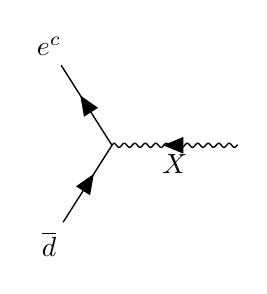
\begin{tikzpicture}
          \begin{feynhand}
            \vertex [particle] (e) at (-0.8,1.26) {$e^c$};
            \vertex [particle] (d) at (-0.8,-1.26) {$\overline{d}$};
            \vertex (x_in) at (0,0);
            \vertex (x_out) at (1.6,0);
            \propag [fermion] (x_in) to (e);
            \propag [fermion] (d) to (x_in);
            \propag [charged boson] (x_out) to [edge label =$X$] (x_in);
          \end{feynhand}
        \end{tikzpicture}
      \end{minipage} &
      \begin{minipage}[b]{0.20\columnwidth}
        \centering
        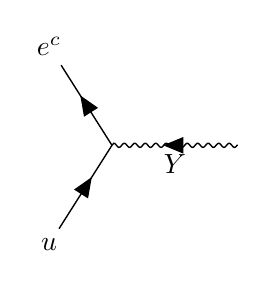
\begin{tikzpicture}
          \begin{feynhand}
            \vertex [particle] (e) at (-0.8,1.26) {$e^c$};
            \vertex [particle] (d) at (-0.8,-1.26) {$u$};
            \vertex (x_in) at (0,0);
            \vertex (x_out) at (1.6,0);
            \propag [fermion] (x_in) to (e);
            \propag [fermion] (d) to (x_in);
            \propag [charged boson] (x_out) to [edge label =$Y$] (x_in);
          \end{feynhand}
        \end{tikzpicture}
      \end{minipage} &
      \begin{minipage}[b]{0.20\columnwidth}
        \centering
        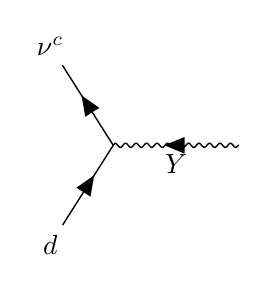
\begin{tikzpicture}
          \begin{feynhand}
            \vertex [particle] (e) at (-0.8,1.26) {$\nu^c$};
            \vertex [particle] (d) at (-0.8,-1.26) {$d$};
            \vertex (x_in) at (0,0);
            \vertex (x_out) at (1.6,0);
            \propag [fermion] (x_in) to (e);
            \propag [fermion] (d) to (x_in);
            \propag [charged boson] (x_out) to [edge label =$Y$] (x_in);
          \end{feynhand}
        \end{tikzpicture}
      \end{minipage}
    \end{tabular}
  \end{center}
  \caption{$X$ボゾン, $Y$ボゾンによるクォークとレプトンの相互作用.}
  \label{fig_X_boson}
\end{figure}
\begin{figure}[ht]
  \centering
  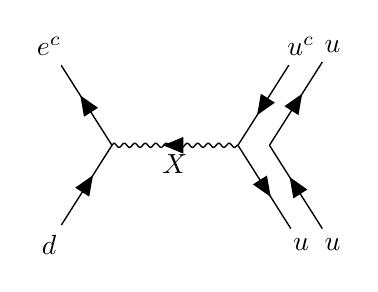
\begin{tikzpicture}
    \begin{feynhand}
      \vertex [particle] (e) at (-0.8,1.26) {$e^c$};
      \vertex [particle] (d) at (-0.8,-1.26) {$d$};
      \vertex (x_in) at (0,0);
      \vertex (x_out) at (1.6,0);
      \vertex [particle] (u) at (2.4,1.26) {$u^c$};
      \vertex [particle] (uc) at (2.4,-1.26) {$u$};
      \vertex (free) at (2.0,0);
      \vertex [particle] (fu_in) at (2.8,-1.26) {$u$};
      \vertex [particle] (fu_out) at (2.8,1.26) {$u$};
      \propag [fermion] (x_in) to (e);
      \propag [fermion] (d) to (x_in);
      \propag [fermion] (u) to (x_out);
      \propag [fermion] (x_out) to (uc);
      \propag [fermion] (fu_in) to (free);
      \propag [fermion] (free) to (fu_out);
      \propag [charged boson] (x_out) to [edge label =$X$] (x_in);
    \end{feynhand}
  \end{tikzpicture}
  \label{fig_X_proton_decay}
  \caption{$X$ボゾンを介した陽子崩壊のファインマン図}
\end{figure}
\subsection{電荷の量子化}
式(\ref{quantum_Q})で述べているが, 標準模型では予言されない電荷の量子化が行える.
これは$SU(5)$大統一理論がクォーク, レプトンを $SU(5)$の単純群で記述し, 式(\ref{GUT-5rep})のように$\overline{\bm{5}}$表現に当てはめることで
\begin{align}
  \mathrm{Tr}Q = 0 \nonumber
\end{align}
と標準模型では与えられない条件を満足させているためである.
\subsection{ワインバーグ角}
標準模型に現れるフェルミオンやゲージ粒子が, $\mathrm{SU(5)}$大統一理論でどのように当てはめられるのかを見てきた.
ゲージ結合定数が大統一スケールで$g_5$と統一されたことにより, 理論的にワインバーグ角を決定することができる.
それを見るために$\mathrm{U(1)_Y}$ゲージ群の結合定数を$SU(5)$の中で規格化する.
フォトン場を$A_\mu$, 中性弱ボゾンを$Z_\mu$とすると
\begin{align}
  D_\mu &\supset \partial_\mu -i\frac{g_5}{2}[W^0 L_{11} + B L_{12}]\nonumber\\
        &\quad=\partial_\mu -i\frac{g_5}{2}[(\sin\theta_W L_{11} + \cos\theta_W L_{12})A_\mu + (\cos\theta_W L_{11} -\sin\theta_W L_{12})Z_\mu]\nonumber\\
        &\quad\equiv \partial_\mu -i[eQA_\mu + g' Q_Z Z_\mu]\nonumber
\end{align}
となる.
このとき, 電荷を表す演算子$Q$は,
\begin{align}
  eQ = \frac{g_5}{2}(\sin\theta_W L_{11} + \cos\theta_W L_{12})\nonumber
\end{align}
と関係する.
一方で電荷演算子はアイソスピン$I_3 = L_{11}$と超電荷$Y=\sqrt{\frac{5}{3}}L_{12}$を用いると
\begin{align}
  Q = L_{11} + \sqrt{\frac{5}{3}}L_{12}\nonumber
\end{align}
とかける.
これらを比較することで,
\begin{align}
  e &= g_5\sin\theta_W\nonumber\\
  g_Y&= \frac{e}{\cos\theta_W}=\sqrt{\frac{3}{5}}g_5 = g_5 \tan\theta_W\label{re_gY}\\
  \sin\theta_W &=\sqrt{\frac{3}{8}}\nonumber
\end{align}
と大統一スケールでの値を予言することができる.
$\sin\theta_W$は標準模型では値を予言することはできなかったが, 大統一理論では予言ができることが示された.


%EOF


% ----- 2nd part -----
%\part{研究の部分}

\chapter{SU(5)大統一理論の拡張模型}
% ---------------------------------------
%
%  Extend to SU(5) GUT
%  extend_SU5.tex
%  Program modified by Yasutoki Takamura
%  Last Modified Jan 23 2025
%
% ---------------------------------------
ここまでで$SU(5)$大統一理論について見ることができた.
電荷の量子化を理論に基づいて自然と説明されることは魅力的である.
一方で, 陽子崩壊やワインバーグ角など現在の実験と整合性の合わない事実も残される.
さらに標準模型の課題を$SU(5)$大統一理論によってすべて解決することができない.
そのため, 高いエネルギースケールで3つの相互作用が統一されるべきという立場を取るならば, 大統一理論を拡張し, 標準模型を超えた物理を探査することが必要となる.

したがって, ここまで見てきたH.Georgi, S.L.Glashowによる$SU(5)$大統一模型を最小$SU(5)$模型と呼び, $SU(5)$模型の拡張方法について例を見る.
\section{SU(5)大統一理論の課題}
\begin{itemize}
  \item ゲージ結合定数の統一\\
        くりこみ群方程式を解くことにより, ゲージ結合定数の大きさのエネルギー依存性を求めることができた.
        大統一理論は高いエネルギースケールではゲージ結合定数は1つに統一されるべきであると考える.
        ところが図\ref{fig:RGE_SM}で見たように, 最小$SU(5)$大統一理論ではゲージ結合定数の大きさは統一されない.
  \item ニュートリノ質量\\
        標準模型を拡張して重たい場を加えてニュートリノ質量を導く方法はあるが, 大統一理論はそのような拡張よりも高いエネルギースケールで成り立つ理論である.
        そのため, 大統一スケールであればそのような拡張を自然と含んだ模型である必要がある.
        最小$SU(5)$大統一理論は標準模型粒子の他に, $T \,(\in \phi_{\bar{\bm{5}}})$ヒッグスと$X,Y$ボゾンを含むが, 右巻きのカイラリティを持つニュートリノ$\nu_R$を含まないため, ニュートリノのディラック型質量項を表すことができない. 
  \item 暗黒物質
  \item 暗黒エネルギー
\end{itemize}
\section{高次元表現を用いた拡張}
場の量子論に基づくと, ゲージ対称性により許される表現は理論に加えることが可能である.
ここでは高次元表現で表される粒子による拡張を与え, それらが現象論的にどのような予言をもたらすのかを見る.
\subsection{45表現ヒッグスを用いた拡張}
大統一理論において, 式(\ref{decon_510})のように基本表現である$\bm{5}$表現から$\bm{45}$表現を考えることができる.
この表現を用いた$\bm{45}$表現ヒッグス$(\phi_{\bm{45}})$ を考える
\cite{framptonEstimateFlavorNumber1979,georgiNewLeptonquarkMass1979}.
これは
\begin{align}
  \left(\phi_{\bm{45}}\right)^{ij}_k = -(\phi_{\bm{45}})^{ji}_k,\quad (\phi_{\bm{45}})^{ij}_i =0 \quad(i,j,k =1,\cdots,5)\nonumber
\end{align}
と
また, $\phi_{\bm{45}}$は次のように分解される.
\begin{align}
  \phi_{\bm{45}} &= \varphi_8 \left(\bm{8}, \bm{2}, \frac{1}{2}\right) \oplus \varphi_{\bar{6}}\left(\overline{\bm{6}}, \bm{3}, -\frac{1}{3}\right) \oplus \varphi_3^T\left(\overline{\bm{3}}, \bm{3}, -\frac{1}{3}\right) \nonumber\\
                 &\qquad\qquad\oplus \varphi_3^D\left( \overline{\bm{3}}, \bm{2}, -\frac{7}{6}\right) \oplus \varphi_3^S\left(\bm{3}, \bm{1}, -\frac{1}{3}\right)\oplus \varphi_{\overline{3}}^S\left( \overline{\bm{3}}, \bm{1}, \frac{4}{3}\right)\oplus H_2\left(\bm{1}, \bm{2}, \frac{1}{2}\right)\nonumber
\end{align}
45表現ヒッグスは真空期待値を
\begin{align}
  \langle (\phi_{\bm{45}})^{j5}_i\rangle = v_{45}\left(\delta^j_i - 4\delta^j_4 \delta_i^4\right),\quad(i,j=1,\cdots 4)
\end{align}
と取ることにより, ゲージ対称性を$SU(3)_c\times U(1)_{em}$へ破る.
\subsection{15表現ヒッグスを用いた拡張}
\begin{align}
  \phi_{\bm{15}} = \Delta \left(\bm{1}, \bm{3}, 1\right) \oplus \widetilde{R_2}\left(\bm{3}, \bm{2},\frac{1}{6}\right)\oplus S\left(\overline{\bm{6}}, \bm{1}, -\frac{2}{3}\right)
\end{align}
と分解できる.
\footnote{
  この記法は\cite{dorsnerPhysicsLeptoquarksPrecision2016}を参考にした.
}
%EOF


% ----- Appendix -----
\appendix
\chapter{群論}
% ---------------------------------------
%
%  Group theory
%  group_theory.tex
%  Program modified by Yasutoki Takamura
%  Last Modified Jan 27 2025
%
% ----------------------------------------
この章では, 大統一理論に必要な数学の内容を非常に簡単にまとめた.
本文でもほとんど触れられているが, 数学の部分のみを取り出してまとめている.
次のことを認め, 話を進める.

$X$を集合とする.
写像$\phi: X\times X \rightarrow X$のことを集合$X$上の演算と言う.
これ以降では$a,b,\in X$に対する写像を$\phi(a, b)$の代わりに$ab$と書く.
\section{群}
群とは次の性質を持つものである.
\begin{dfn}[群]
  $G$を空ではない集合とする. 集合$G$上で演算が定義されており, 次の性質を満たすとき, $G$を群と言う.
  \begin{enumerate}
    \item 単位元と呼ばれる$e\in G$が存在し, 全ての$a\in G$に対して$ae=ea=a$となる.
    \item すべての$a\in G$に対し, $b\in G$が存在し, $ab=ba=e$となる. この元$b$は$a$の逆元と呼ばれ, $a^{-1}$と書く.
    \item すべての$a, b, c \in G$に対して, $(ab)c=a(bc)$が成り立つ.
  \end{enumerate}
\end{dfn}
特に, 性質3. は結合法則と呼ばれている.
群の元$a, b\in G$に対して$ab=ba$が成り立つとき, $a, b$は可換である.
$G$の任意の元$a, b$が可換なら, $G$を可換群(Abel群)と呼ぶ.
\section{Lie群}
Lie群は連続なパラメータにより特徴づけられる群であり, 生成子$t^a$によって
\begin{align}
  g(\alpha) = \exp(i\alpha^a t^a)
\end{align}
となる.
この生成子$t^a$は, リー括弧によって
\begin{align}
  [t^a, t^b] = if^{abc}t^c
\end{align}
を満たす.
ここで, $f^{abc}$はリー代数の構造定数である.
\section{表現}
表現とは, 群を行列に対応させる写像である.
この写像は$\mathcal{R}: G\rightarrow GL(n)$で定義される.
表現の次元は行列の次元と等しい.


%EOF



% ----- Bibliography -----
\bibliographystyle{junsrt}
\bibliography{
bibs/GUT.bib,
bibs/Standard_Models.bib,
bibs/CS_Equation.bib,
bibs/Glashow_Weinberg.bib,
bibs/QCD.bib,
bibs/beta_function.bib,
bibs/Experimental.bib,
bibs/neutrino_oscillation.bib,
bibs/neutrino_oscillation_th.bib,
bibs/Leptoquark.bib,%
bibs/SU5_45Higgs.bib
}


\end{document}
%EOF
